\part{
    Potential Surface
    \\
    \large{Establishing What's Possible}
}
\label{sec:PotentialSurface}

\chapter{Initial Explorations}

As stated in the introduction, every person responds to lifting differently. This chapter is concerned with finding and establishing the limits of a given lifter within the context of a single exercise.

There are many limiting factors that need to be considered. How many reps can be done per set? How many sets can be done per exercise? What weight can the user lift given a particular amount of sets and reps? How much effort should the lifter exert to perform those sets and reps at the given weight? The answers to these questions form the thought process for the rest of the section.

When performing a single exercise, there are generally six things that dictate what is done:
\begin{enumerate}
    \item What exercise is being performed
    \item The number of sets being performed for a particular exercise
    \item The number of reps being performed for each set
    \item The weight each rep should be performed at
    \item The amount of effort expected to be exerted on each set
    \item The lifters current abilities
\end{enumerate}

The exercise being performed is largely dependent on what goals the lifter is pursuing as well as what weaknesses the lifter has. Due to the complexity of exercise selection as well as it's independence from the last five items on the list, it is explored in greater detail in a separate chapter. The last five items on that list have a large amount of dependence upon each other, and the relationship among them will be established in this chapter.

\section{Intuitive Relationships Between Variables}
\label{sec:PotentialSurfaceIntuitiveRelationshipsBetweenVariables}

The ultimate goal of this part of this book is to create a surface that represents what is possible for a lifter to do. To accomplish this, the nature of the surface must first be explored. This can be done by looking at the data as well as applying already established facts about lifting. Briefly, it is worth mentioning why this process is being done manually instead of through other processes common in machine learning. When processes similar to machine learning are conducted the nature of the surface is unknown, which can lead to problems when trying to verify the surface has the desired behavior. This is a known issue with machine learning, with it often being compared to a black box. Understanding the behavior of the surface is important to be able to constrain it so that it will not instruct a lifter to perform impossible tasks that will likely lead to injury. Being able to prove that the surface will not stray into the impossible is very important, and will require understanding of all the variables that define its behavior.

Many of the variables that need to be looked at are extremely interdependent on each other. Sets and reps depend on each other, with an increase in one generally requiring a decrease in the other. Intensity depends on sets and reps, with higher intensities requiring possibly less sets and possibly reps. Going back to the relation to sets and reps however, if sets increases and weight decreases then reps could increase, decrease, or remain the same. Effort depends on intensity as well as sets and reps... The point should be clear. Trying to define behaviors based on all of these interdependent variables quickly gets out of hand. Instead of doing this, the behaviors of each variable will be defined in relation to volume where each variable can be viewed independently from the others. Doing this also allows more abstract properties to be considered, such as volume tolerance. With that said, the rest of this section outlines the desired behaviors of the surface.

\subsection{Property 1: Volume and Intensity}
\label{sec:PotentialSurfaceIntuitiveRelationshipsBetweenVariablesVolumeAndIntensity}

A lifter has a \textit{volume tolerance}, which represents there work capacity. Given a certain volume tolerance, the only five variables that can change are weight, intensity, effort, sets, and reps. This is demonstrated in equations \ref{eq:BaseVolumeEquation} and \ref{eq:IntensityBasedVolumeEquation}.

Weight and intensity are synonymous through the lens of volume, as the total amount of weight lifted is calculated regardless of the differing parameters. Looking at equations \ref{eq:BaseVolumeEquation} and \ref{eq:IntensityBasedVolumeEquation} it is natural to assume volume will increase with increased weight and intensity. Mathematically, this makes sense, but the limits of the human body need to be considered. As intensity approaches $100\%$ more effort is required to maintain the same amount of volume. Because effort is limited, volume will necessarily decrease at higher weights, to a point where it reverses the increase in volume from the increase in weight. An example may make this clearer. At $100\%$ intensity a lifter can realistically expect to obtain a maximum volume near there 1RM, as shown in equation \ref{eq:VolumeWithDiffereingIntensities1}. \footnote{The actual volume reached as intensity increases may be slightly more or less than the lifters 1RM because of other limiting factors such as effort and fatigue, which will be discussed in the following sections. As the next sections will explore, if effort is maximized and fatigue is minimized then the maximum possible volume should be expected to be at or above the lifters 1RM.} At $50\%$ intensity, all it takes is two reps to match the volume performed at $100\%$ intensity, which is shown in equation \ref{eq:VolumeWithDiffereingIntensities2}. At $50\%$ intensity, far more than one set of two reps can be performed, making it easy to surpass the volume done at $100\%$ intensity. The data discussed in chapter \ref{sec:DataSection} has many examples of this.

\begin{subequations}
    \begin{align}
        \label{eq:VolumeWithDiffereingIntensities1}
        v_{I=1}=&v(s=1,r=1,w=l_{1RM})=l_{1RM} \\
        \label{eq:VolumeWithDiffereingIntensities2}
        v_{I=0.5}=&v(s=1,r=2,w=0.5l_{1RM})=l_{1RM}
    \end{align}
\end{subequations}

The fact that volume diminishes at higher intensities cannot be stressed enough, as it breaks any intuition gathered from equations \ref{eq:BaseVolumeEquation} and \ref{eq:IntensityBasedVolumeEquation}. These equations, serve as a way to \textit{measure} volume, not as a proxy to determine what is possible. These equations have no regard to the limitations of the human body. It is common knowledge among strength coaches that if you want to increase volume sets and reps need to be increased, not weight.

Now, for lower intensities, it is tempting to say that as weight approaches $0$ volume will linearly decrease to $0$. Again, while mathematically true, the human body does not follow a linear decrease in volume. When weight diminishes it become easier to lift the weight. Common knowledge dictates that performing some small, light task it can be done many times. Now, this does not come at no cost, as when intensity decreases more endurance is required. However, generally speaking, the human body is made for endurance. Running for long distances is one of our strengths thanks to evolution. What this means for lifting is that as weight decreases so many more sets and reps can be done that the decrease in volume from the decrease in weight is overcome. Volume cannot indefinitely increase, there is a limit of course. This limit is known as the lifters volume tolerance. As weight decreases more sets and reps can be done until this limit is reached.

Given the above discussion the following properties can be gathered:

\begin{itemize}
	\item Property 1.a:  As intensity approaches $100$\%  volume will decrease until it is near the lifters 1RM.
	\item Property 1.b: As intensity approaches $0$\% volume will approach some plateau, or asymptote in mathematical terms. The exact value of the plateau will need to be found from the data.
\end{itemize}

To confirm this behavior the data will need to be considered. Looking at figure \ref{fig:IntensityVsVolumeGraph}, it does not demonstrate this pattern very well. The first item of the above list is visible in the data as volume decreases past $80$\% intensity until it reaches the volume equivalent to a 1RM. The second item of the list however does not appear to be present in the data. Instead of reaching a rough plateau it reaches a peak and drops off linearly past the peak. This seemingly goes against the pattern that was discussed when considering the limits of the human body.

\begin{figure}
    \centering
    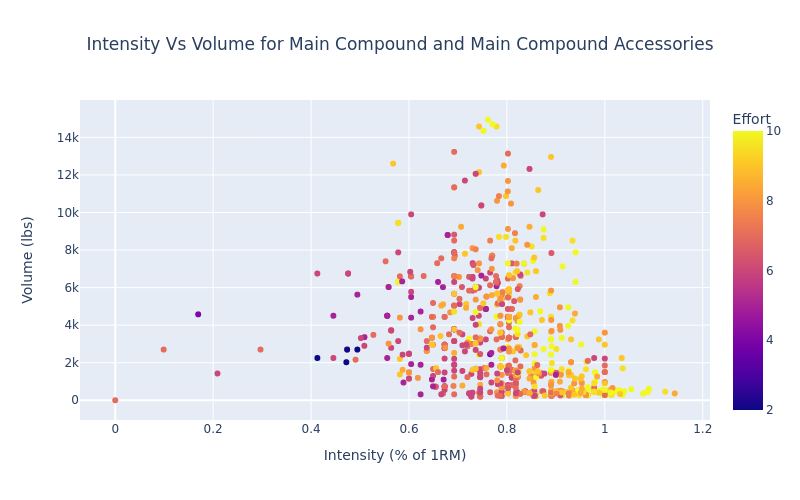
\includegraphics[scale=0.55]{images/ch3/IntensityVsVolume.png}
    \caption{A graph comparing intensity and volume. Note how there is a clear peak in volume between $60\%$-$80\%$.} 
    \label{fig:IntensityVsVolumeGraph}
\end{figure}

The explanation for the peak in volume is rather simple. It is due to the data being collected by a powerlifter, a sport that does not require much in the way of endurance, which skews the data as a result. This skewing of the data will come up again and be discussed more thoroughly in the next section, which is concerned with volume and effort.


\subsection{Property 2: Volume and Effort}
\label{sec:PotentialSurfaceIntuitiveRelationshipsBetweenVariablesVolumeAndEffort}

The next question is what happens when effort increases or decreases across all intensities. As effort increases more sets will be able to be completed, more reps will be able to be completed in each set, or more weight will be able to be lifted. If the increase in effort is large enough, some combination of sets, reps, and weight could all increase. The opposite is true if effort decreases. Again, it should be clear that sets and reps are directly proportional to volume, implying an increase in either one will increase volume. Putting all of this together, as effort increases volume will increase and as effort decreases volume will decrease.

\begin{figure}
    \centering
    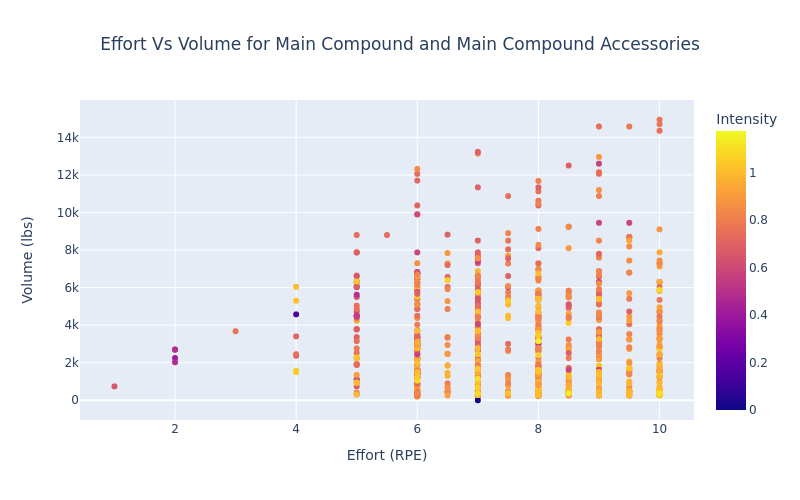
\includegraphics[scale=0.55]{images/ch3/EffortVsVolume.png}
    \caption{A graph comparing effort and volume. Note how there appears to be no correlation between volume and effort.}
    \label{fig:EffortVsVolumeGraph}
\end{figure}
\begin{figure}
    \centering
    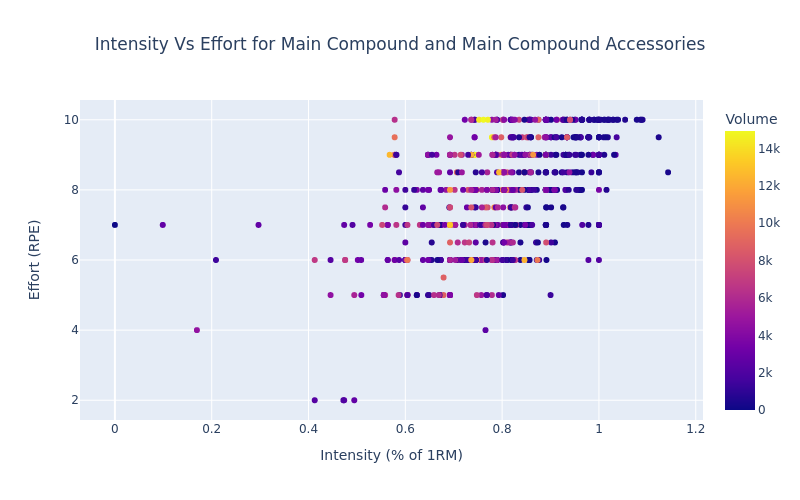
\includegraphics[scale=0.55]{images/ch3/IntensityVsEffort.png}
    \caption{A graph comparing effort and intensity. Note how the intensity tends to increase with higher effort values. This is the result of a powerlifters goal to increase a 1RM.}
    \label{fig:EffortVsIntensity}
\end{figure}

However, in figure \ref{fig:EffortVsVolumeGraph}, which compares volume and effort, volume does not seem to correlate with effort as previously mentioned. Only at the extreme values of each RPE rating does the behavior seem to follow. When looking at the graph as a whole there appears to be no pattern. The reason for this is the same as the previous section. A powerlifter collected the data and the goal of a powerlifter, above all, is to maximize weight. This goal can be seen in figure \ref{fig:EffortVsIntensity}, where intensity positively correlates with effort. What figure \ref{fig:EffortVsIntensity} is saying is that as effort increases the lifter chose to increase weight over sets and reps. Increasing weight, or intensity, will not increase volume as much as if sets and reps were increased due to the previously established fact that volume at higher intensities is necessarily limited by effort. This is a clear bias in the data set, and explains why volume is seemingly constant in figure \ref{fig:EffortVsVolumeGraph}. Given a sport that is more concerned with rep maxes, such as Crossfit, the effort vs intensity graph would level out because lower intensities would be pushed for as many reps as possible, creating maximal effort sets with lower intensities. \footnote{This is a perfect example to demonstrate how effort and intensity are two different concepts.} In order to have maximal effort sets with lower intensities either sets, reps, or both sets and reps will need to increase, forcing volume to increase considerably and restoring the correlation between effort and volume previously discussed.


\subsection{Property 3: Volume and Fatigue}
\label{sec:PotentialSurfaceIntuitiveRelationshipsBetweenVariablesVolumeAndFatigue}

Fatigue will necessarily limit volume. The reasoning behind this is simple, the more fatigued you are the less work you can safely do. There can be many sources of fatigue but they will all have the same effect of limiting volume. At the extreme, fatigue will make it so no work can be done at all and hence $0$ volume can be tolerated. This is a state that should be be avoided at all costs, as it is the epitome of over training. When fatigue is at a minimum a lifter will be able to reach there highest potential in there current state. Note that fatigue cannot add to a lifters abilities, it can only diminish them. This is true regardless of effort. No matter how much effort a lifter puts into a set, they would have always been able to lift more weight had they been less fatigued.


\subsection{Property 4: Sets and Reps}
\label{sec:PotentialSurfaceIntuitiveRelationshipsBetweenVariablesSetsAndReps}

With effort, intensity, and fatigues relation to volume being explored, sets and reps are all that's left. It may be tempting to conclude that volume should be constant given a particular weight and effort. This conclusion can be reached by looking at equations \ref{eq:BaseVolumeEquation} and \ref{eq:IntensityBasedVolumeEquation}, where once the weight and effort are known sets and reps would just vary inversely to ensure volume remains constant. Again, while mathematically true, the limits of the human body need to be considered. Evidence that the relationship between sets and reps is not perfectly inverse is shown in figure \ref{fig:SetsVsReps}, where a slight drop in sets from the expected inverse pattern is seen. This favoritism between sets and reps will of course mean volume is no longer constant given a particular intensity and effort, and as such will be known as the \textit{volume skew}.
%This can be attributed to a lack of \textit{endurance}, where sets with a greater number of reps  require more endurance than sets with less reps. Powerlifters are eternally known for having no endurance, so it should come as no surprise that they will favor more sets over reps.

\begin{figure}[h]
    \centering
    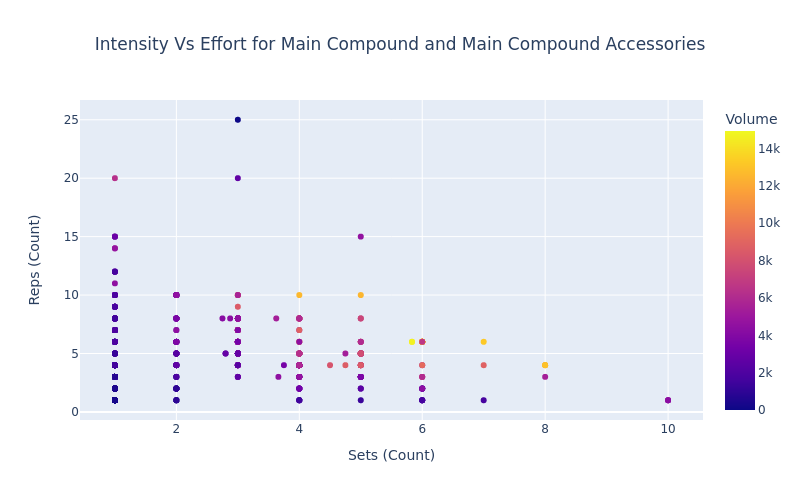
\includegraphics[scale=0.55]{images/ch3/SetsVsReps.png}
    \caption{A graph comparing average reps and sets for main compound and main compound accessory lifts. Note how the relationship is not perfectly inverse. Don't assume any volume skew seen in this graph is necessarily true for all the data, as this plot shows many exercises over a large time span. Finding volume skew will eventually need to be done on a per exercise basis across time.}
    \label{fig:SetsVsReps}
\end{figure}

By this point it should be obvious the crux of the problem in question will require finding a lifters volume tolerance across intensity and effort, as well as the lifters volume skew between sets and reps. In order to solve this problem, a surface will need to be found that exhibits the appropriate behaviors and then that surface will need to be fitted to the data. These surfaces will be called \textit{potential surfaces}, because they represent a lifters potential performance. It is important to conceptualize that every combination of sets, reps, weight, and effort defined by a potential surface is theoretically possible for a lifter to complete. This is the foundation this entire book will build off of.


\section{Linear Regression and Time Series Problems}
\label{sec:PotentialSurfaceLinearRegressionAndTimeSeriesProblems}

Before moving forward with the goal of finding a surface of best fit using the data set and linear regression, the limits of linear regression need to be considered. Looking at the data set, it should be clear that it is a time series: the data points are collected over time, and data points nearer in time have greater importance than data points farther away in time. Linear regression assumes that all the data points are uncorrelated, which is clearly untrue with time series data. To reconcile the differences between working with linear regression and a time series data set, two things can be done.

The first step that can be taken is to limit the time frame that linear regression is run over. Sets, reps, volume, and the volume skew can all vary through time, but not necessarily in direct linear relation to time. As an example of this, consider seasonal training, which some powerlifters choose to employ. In the off season intensities will drop, volume will increase, and the emphasis on training may shift to hypertrophy over strength. In the on season intensities will increase, volume will necessarily decrease, and the emphasis on training will shift to strength over hypertrophy. This will result in shifts in the number of sets and reps being done over time. To capture these changes over time several techniques can be used. The exact equations that determine what data points are included and to what extent they are considered will be discussed more in chapter \ref{sec:TimeFrame}. That being said, some notation is required to continue. The general notation used to show which data points will be used when performing linear regression is shown in equation \ref{eq:TimeFrame}. The exact length of the time frame, $t_f$, along with any other specifics, will be discussed in chapter \ref{sec:TimeFrame}. Throughout the rest of this book equation \ref{eq:TimeFrame} will be written short hand as $t_i\in \{ T \}$ In an effort to save space.

\begin{equation}
    \label{eq:TimeFrame}
    %t_t\le t_i\le t_t+t_f
    t_i \in\{ t_t, t_t+1,\dots,t_t+t_f \}
    \equiv t_i \in \{ T \}
\end{equation}
\centerline{where}
\begin{equation*}
    \begin{split}
        t_i &\equiv \text{The time component of an arbitrary data point }i \\
        t_t &\equiv \text{An arbitrary target time} \\
        t_f &\equiv \text{The time frame linear regression will be run over} \\
        T & \equiv \text{A shorthand notation representing the set of all allowed times}
    \end{split}
\end{equation*}

The second step that can be taken is to remove weights correlation with time. Weight correlating with time makes intuitive sense, as the goal of a powerlifter is to continually increase weight over time. As an example, say a lifter starts out with a 1RM of $300$ lbs on squat, but through training is able to increase that weight over time to $800$ lbs. It should be obvious from the example that weight has a positive correlation with time. To fix this, weight will be replaced by intensity. This will remove the correlation with time because intensity is calculated using an exercises 1RM, which itself changes with time, canceling out any effects from an increase in weight through time. To show this the previous example will be used again. Despite weight increasing over time, intensity would generally be limited to the range $0\le I\le 1$ because the lifter would set new 1RM's over time, thereby forcing the intensities to be generally less than $1$.

Having an accurate tracking of a lifters 1RM over time becomes an important dependence for the model now that weight is replaced by intensity. For a powerlifter, this is generally not a problem as a lifts 1RM is usually tested once a macrocycle. Problems arise however when things like injuries, or other unplanned problems occur. During these situations a lifters 1RM is not known and can change rapidly or extremely slowly over time. A solution to problems like this will be explored in sections \ref{sec:TimeFrameDynamicTimeFrameAnalysis} and \ref{sec:TimeFrameInjuriesAndChanges}.


\section{The Effort-Fatigue Model}
\label{sec:PotentialSurfaceEffortFatigueModel}

While exploring the intuitive relationships between variables a large amount of emphasis was placed on volume, with most variables being discussed in relation to volume. Despite this, this section is more concerned with how the surface is going to be defined, which will not involve directly involve volume. Instead, the general idea of how the surfaces presented in the next couple sections were conceptualized will be discussed. Within each surfaces chapter, there will be a discussion about how the surface abides by the intuitive behaviors, if at all.

With that, the starting point of every surface is amusingly simple, and can be summed up in the following phrase: Performance is effort diminished by fatigue. To be more specific, performance is equal to total effort diminished by total fatigue. It is tempting to say that, for a powerlifter, performance is simply the weight that is lifted, making $P=w$. However, remembering that these surfaces will eventually be fitted to the data using linear regression and after the discussion in section \ref{sec:PotentialSurfaceLinearRegressionAndTimeSeriesProblems} it should be clear that intensity should be used in the place of weight to measure performance, making $P=I$. Equation \ref{eq:PerformanceProxy} shows an approximate form for the effort-fatigue model.

\begin{equation}
	\label{eq:PerformanceProxy}
	\begin{split}
			P &\hat{=} E_{tot}\hat{-}F_{tot} \\
			I &\hat{=} E_{tot}\hat{-}F_{tot}
	\end{split}
\end{equation}

The $\hat{=}$ symbol in this case means "something like". It is chosen to mean this over something like the $\approx$ symbol because these equations are approximations in the loosest sense. The equations in this section merely form a rough template for later chapters to fully realize. The $\hat{-}$ symbol means "diminished by". The true mathematical interpretation of the $\hat{-}$ symbol is left for future chapters to define.

After performance, total effort is the next easiest term to understand as it directly correlates to how effort was discussed in section \ref{sec:CommonTermsSection}. The only effort that can be applied is by the lifter themselves, no other external factor can 'add effort' to a lifters workout. \footnote{An argument could be made for pre-workout, sugar rushes, a lifter 'getting in there head', or adrenaline dumps 'adding effort', but these are only tools to help a lifter to exert more effort, not tools to generate more effort in and of themselves. Even with these tools, at the end of the day, the effort still has to come from the lifter themselves.} Given this, $E_{tot}$ can be nicely summed up in equation \ref{eq:TotalEffort}. Because there is only one source of effort, a true equality sign can be used. $\epsilon_1$ is a constant that will need to be found after performing linear regression on whatever concrete representation of the surface the next few chapters decide upon.

\begin{equation}
	\label{eq:TotalEffort}
	E_{tot}=\epsilon_1 E
\end{equation}

Total fatigue is more complicated, as there are several different types of fatigue that contribute to it's total. Given the four different types of fatigue listed in section \ref{sec:ModifiedFatigueCategories}, total fatigue can be represented as follows. Total fatigue is more open to intrepretation than total effort, hence the $\hat{=}$ symbol.

\begin{equation*}
	F_{tot} \hat{=} \epsilon_2 F_l+\epsilon_3 F_w+\epsilon_4 F_e+\epsilon_5 F_s
\end{equation*}

Section \ref{sec:AugmentedDataSet} introduced indexes to represent inter-workout and inter-exercise fatigue. These data points can be directly used in the above equation, however as discussed in section \ref{sec:AugmentedDataSet} the index values only represent the fatigue present before the exercise is performed. The fatigue generated from the current exercise needs to be considered to avoid scenarios where the lifter fails a lift due to being too fatigued to make it through the entire exercise. This is where inter-set fatigue matters. Inter-set fatigue will increase in proportion to to total number of reps done. Two additional terms can be added to measure the fatigue generated from sets and reps individually.

\begin{equation*}
	F_{tot} \hat{=} \epsilon_2 F_l+\epsilon_3 F_w+\epsilon_4 F_e+\epsilon_5 sr+\epsilon_6 s+\epsilon_7 r
\end{equation*}

Finally, the approximate form of the effort-fatigue model can be defined, and is shown in equation \ref{eq:PotentialSurfaceEquation}. Again, this may seem like a finished equation, but remember this is just a template. The surfaces in the next several chapters will create final equations to concretely realize the ideas of the effort-fatigue model, apply constraints, and enforce desired behavior. These equations may take very different forms, but the general idea of the effort-fatigue model still stands behind them.

\begin{equation}
	\label{eq:PotentialSurfaceEquation}
	\begin{split}
		I & \hat{=} E_{tot}\hat{-}F_{tot} \\
		I & \hat{=} \epsilon_1 E\hat{-}\left( 
			\epsilon_2 F_l+\epsilon_3 F_w+\epsilon_4 F_e+\epsilon_5 sr+\epsilon_6 s+\epsilon_7 r
		\right)
	\end{split}
\end{equation}

Before going to the next chapters, it is worth mentioning that latent fatigue will be discussed in chapter \ref{sec:}. It has it's rightful place in the potential surface, but it's implications are so broad that they need a chapter of there own. Until chapter \ref{sec:} the effects from latent fatigue will not be considered. For now, think of it as though $\epsilon_2$ were set to $0$. 


\chapter{Surface 1: The Basic Surface}
\label{sec:PotentialSurfaceTheBasicSurface}

The first surface to explore takes the effort-fatigue model in and makes as few changes as possible, treating the $\hat{-}$ symbol to mean literal subtraction. The first change it makes is to center the surface at $(s=1,r=2,I=\epsilon)$ so that the peak in intensity occurs with one set of one rep, matching the lifters 1RM. Doing this will require an error term to be added, represented by $\epsilon$. The next, and most substantial change, is to total fatigue. The discussion in section \ref{sec:PotentialSurfaceIntuitiveRelationshipsBetweenVariables} needs to be considered. One of the main takeaways from that section is that volume is limited by effort at high intensities. If the total fatigue template presented by the effort-fatigue model is taken as a literal equation, volume will not have the correct behavior as intensity approaches $100$\%. Namely, there will not be diminishing returns in volume as intensity increases because all the relationships with sets and reps are either linear or a linear combination of both of them. To correct for this, the terms containing sets and reps will be squared, creating diminishing returns to volume with respect to intensity that can be adjusted through the constant in front of each term. \footnote{Yes, there are more flexible ways to do this, but using those ways would make it so linear regression could not be performed due to the multiplicative combinations of constants.} With these changes, the total fatigue equation for the basic surface is shown below. 

\begin{equation*}
	F_{tot} = \epsilon_2 F_l+\epsilon_3 F_w+\epsilon_4 F_e+\epsilon_5 (s-1)^2(r-1)^2+\epsilon_6 (s-1)^2+\epsilon_7 (r-1)^2
\end{equation*}

The final form of the basic surface is shown in equation \ref{eq:BasicSurfaceEquation}. Several constraints are applied to the constants, the reasoning of which will be discussed later in the chapter, but the general idea behind them is to limit the surface to behavior that makes sense for the problem at hand. This equation attempts to fully realize all of the intuitive relationships discussed in section \ref{sec:PotentialSurfaceIntuitiveRelationshipsBetweenVariables}. Which intuitive relationships it fulfills and which it does not will be the topics of sections \ref{sec:PotentialSurfaceAnalysisOfProperty2}-\ref{sec:PotentialSurfaceAnalysisOfProperty4}.

\begin{minipage}{\textwidth}
	\begin{equation}
		\label{eq:BasicSurfaceEquation}
		\begin{split}
			I & =\epsilon+\epsilon_1 E-\left( 
				\epsilon_2 F_l+\epsilon_3 F_w+\epsilon_4 F_e+\epsilon_5 (s-1)^2(r-1)^2+\epsilon_6 (s-1)^2+\epsilon_7 (r-1)^2
			\right)
		\end{split}
	\end{equation}
	\centerline{where}
	\begin{equation*}
	    \begin{split}
	        E & \in \{ 1,1.5,2,2.5, \dots ,10 \} \\
	        \epsilon, \epsilon_1, \epsilon_2, \epsilon_3, \epsilon_4, \epsilon_5,\epsilon_6,\epsilon_7 & > 0 \\
	    \end{split}
	\end{equation*}
\end{minipage}

To run linear regression the error equation is needed, which is shown below.

\begin{equation*}
    E_{rr}=\sum_{
            \substack{i=0\\ t_i\in \{ T \}}
        }^n \left(
        I_i
        -\epsilon
        -\epsilon_1 E_i
        +\epsilon_2 F_{l,i}
        +\epsilon_3 F_{w,i}
        +\epsilon_4 F_{e,i}
        +\epsilon_5 (s_i-1)^2(r_i-1)^2
        +\epsilon_6 (s_i-1)^2
        +\epsilon_7 (r_i-1)^2
    \right)^2
\end{equation*}

To minimize the error, the partial derivatives of each unknown constant need to be found and each one is set equal to zero. An example with $\epsilon$ is shown below.

\begin{equation*}
    \begin{split}
        \frac{\partial E_{rr}}{\partial \epsilon}=
        \frac{\partial}{\partial \epsilon}\sum_{
                \substack{i=0\\ t_i\in \{ T \}}
            }^n \left(
            I_i
            -\epsilon
            -\epsilon_1 E_i
            +\epsilon_2 F_{l,i}
            +\dots
            %+\epsilon_3 F_{w,i}
            %+\epsilon_4 F_{e,i}
            %+\epsilon_5 (s_i-1)^2(r_i-1)^2
            +\epsilon_6 (s_i-1)^2
            +\epsilon_7 (r_i-1)^2
        \right)^2&=0\\
        -2\sum_{
                \substack{i=0\\ t_i\in \{ T \}}
            }^n \left(
            I_i
            -\epsilon
            -\epsilon_1 E_i
            +\epsilon_2 F_{l,i}
            +\dots
            %+\epsilon_3 F_{w,i}
            %+\epsilon_4 F_{e,i}
            %+\epsilon_5(s_i-1)^2(r_i-1)^2
            +\epsilon_6(s_i-1)^2
            +\epsilon_7(r_i-1)^2
        \right)&=0\\
        \epsilon \sum_{\substack{i=0\\ t_i\in \{ T \}}}^n 1 
        +\epsilon_1 \sum_{\substack{i=0\\ t_i\in \{ T \}}} E_i
        -\epsilon_2 \sum_{\substack{i=0\\ t_i\in \{ T \}}} F_{l,i}
        -\dots
        %-\epsilon_3 \sum_{\substack{i=0\\ t_i\in \{ T \}}} F_{w,i}
        %-\epsilon_4 \sum_{\substack{i=0\\ t_i\in \{ T \}}} F_{e,i}
        %-\epsilon_5 \sum_{\substack{i=0\\ t_i\in \{ T \}}}^n (s_i-1)^2(r_i-1)^2
        -\epsilon_6 \sum_{\substack{i=0\\ t_i\in \{ T \}}}^n (s_i-1)^2
        -\epsilon_7 \sum_{\substack{i=0\\ t_i\in \{ T \}}}^n (r_i-1)^2
        &=
        \sum_{\substack{i=0\\ t_i\in \{ T \}}}^n I_i\\
    \end{split}
\end{equation*}

After a similar process is carried out for each unknown constant, equation \ref{eq:LinearRegMatrixEquation} can be used, and the unknown constants can be solved for.

\begin{equation}
    \label{eq:LinearRegMatrixEquation}
	\mathbf{Ax=b}
\end{equation}
\centerline{where}
\begin{equation*}
    \mathbf{A}=\left[
    \begin{matrix}
        \sum_{i=0}^n 1 &
        \dots &
        -\sum_{\substack{i=0\\ t_i\in \{ T \}}}^n (r_i-1)^2 \\

        \sum_{\substack{i=0\\ t_i\in \{ T \}}}^n  E_i &
        \dots &
        -\sum_{\substack{i=0\\ t_i\in \{ T \}}}^n E_i (r_i-1)^2\\

        \vdots &
        \ddots &
        \vdots \\
        
        \sum_{\substack{i=0\\ t_i\in \{ T \}}}^n (r_i-1)^2 &
        \dots &
        -\sum_{\substack{i=0\\ t_i\in \{ T \}}}^n (r_i-1)^4
    \end{matrix}
    \right]
\end{equation*}
\begin{equation*}
    \mathbf{x}=\left[
    \begin{matrix}
        \epsilon \\ \epsilon_1 \\ \vdots \\ \epsilon_7
    \end{matrix}
    \right]
\end{equation*}
\begin{equation*}
    \mathbf{b}=\left[
    \begin{matrix}
        \sum_{\substack{i=0\\ t_i\in \{ T \}}}^n I_i \\
        \sum_{\substack{i=0\\ t_i\in \{ T \}}}^n I_i E_i \\
        \vdots \\
        \sum_{\substack{i=0\\ t_i\in \{ T \}}}^n I_i(r_i-1)^2 
    \end{matrix}
    \right]
\end{equation*}

With equations \ref{eq:PotentialSurfaceEquation} and \ref{eq:LinearRegMatrixEquation}, this surface is fully defined. After fitting the surface to the data discussed in chapter \ref{sec:DataSection}, graphs similar to the ones shown in figure \ref{fig:SquatPotentialSurfaceAcrossEffort} can be created. A full set of potential surface graphs for squat, bench, and deadlift across effort levels $5-10$ are available in appendix \ref{sec:AppendixA}. Many of the relationships discussed in section \ref{sec:PotentialSurfaceIntuitiveRelationshipsBetweenVariables} are concerned with volume. To give some intuition for volume before moving on, equation \ref{eq:IntensitySubedInVolume} is the result of solving the potential surface for $I$ and substituting it in equation \ref{eq:IntensityBasedVolumeEquation}. The graphs shown in figure \ref{fig:SquatPotentialSurfaceVolumeAcrossEffort} show the volume surface generated from this potential surface.

\begin{equation}
    \label{eq:IntensitySubedInVolume}
    \begin{split}
    		v = & srI \\
    			= & sr \left( 
    			\epsilon+
    			\epsilon_1 E-
    			\epsilon_2 F_l-
    			\epsilon_3 F_w-
    			\epsilon_4 F_e-
    			\epsilon_5(s-1)^2(r-1)^2-
    			\epsilon_6(s-1)^2-
    			\epsilon_7(r-1)^2
    		\right)
    \end{split}
\end{equation}

\begin{figure}[htbp]
    \centering
    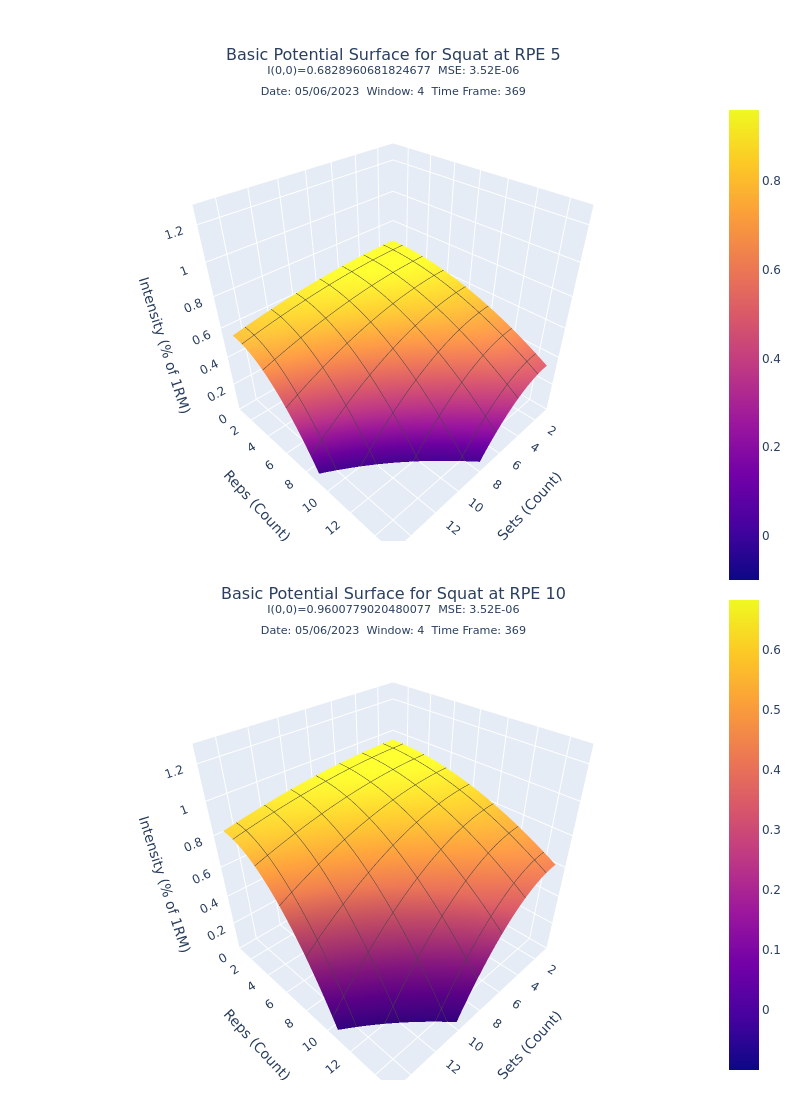
\includegraphics[scale=0.55]{images/ch3/PotentialSurface/DualSquat.Effort[5,10].basic.png}
    \caption{The potential surface fitted to squat data at various effort levels. The window and time frame values will be discussed in chapter \ref{sec:TimeFrame}. For now, the $I(0,0)$ and MSE values are the most important.}
    \label{fig:SquatPotentialSurfaceAcrossEffort}
\end{figure}

\begin{figure}[htbp]
    \centering
    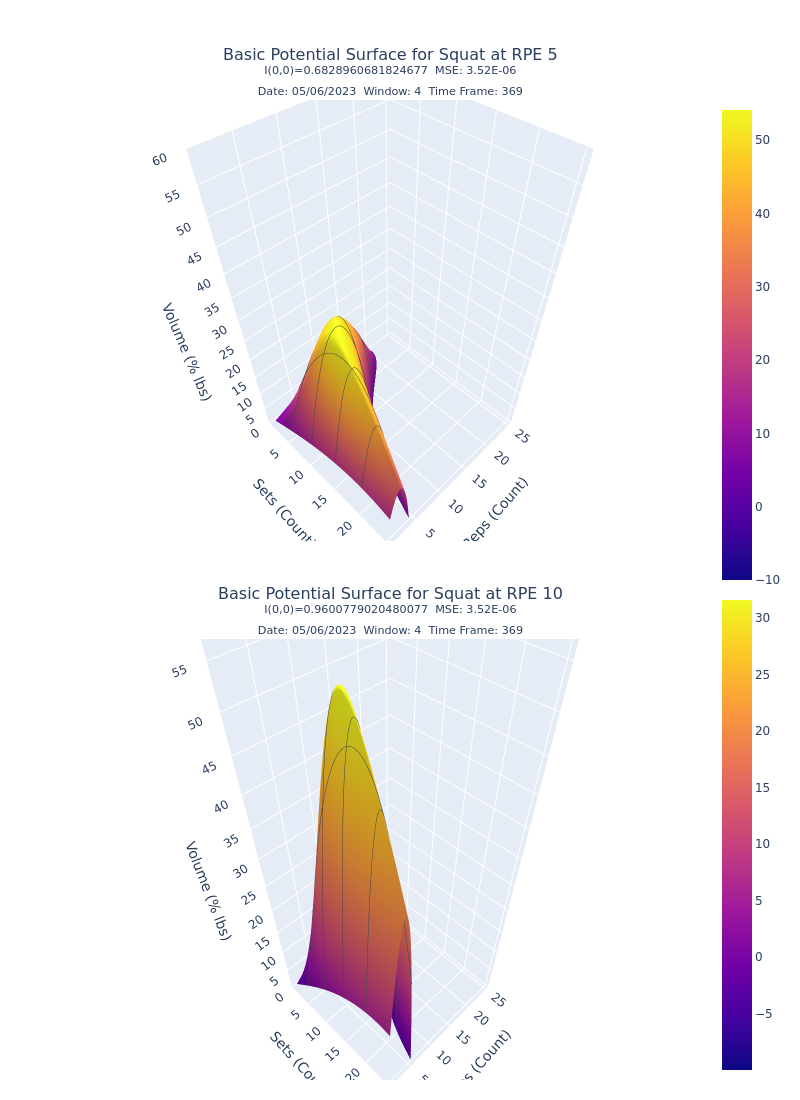
\includegraphics[scale=0.55]{images/ch3/Volume/DualSquat.Effort[5,10].basic.png}
    \caption{The volume surface resulting from the potential surface fitted to squat data at various effort levels.}
    \label{fig:SquatPotentialSurfaceVolumeAcrossEffort}
\end{figure}

\section{Analysis of Property 1.a: Volume and Intensity}
\label{sec:PotentialSurfaceAnalysisOfProperty1a}

Property 1.a is that volume should approach the lifters 1RM as intensity increases. To prove this two things need to happen. It needs to be proven that equation \ref{eq:BasicSurfaceEquation} has a single global maximum and no minimum. This maximum should equal the lifters current 1RM. Given that this is the case, it then needs to be proven that equation \ref{eq:IntensitySubedInVolume} has a  minimum at the same point that equation \ref{eq:BaseIntensityEquation} has it's maximum. This minimum also needs to equal the value of equation \ref{eq:BaseIntensityEquation} at its maximum. Given all this, it can be said that the basic surface exhibits property 1.a because volume has a minimum at the same point where intensity has a global maximum, meaning intensity increases from all directions to that point where volume has a value equal to the lifters current 1RM.

To begin, the maximum of equation \ref{eq:BaseIntensityEquation} needs to be found. This will require the gradient of that function, shown below.

\begin{equation*}
	\nabla I =
	\left[
	\begin{matrix}
		\frac{\partial I}{\partial E} \\
		\frac{\partial I}{\partial F_l} \\
		\frac{\partial I}{\partial F_w} \\
		\frac{\partial I}{\partial F_e} \\ 
		\frac{\partial I}{\partial s} \\
		\frac{\partial I}{\partial r} \\
	\end{matrix}
	\right] =
	\left[
	\begin{matrix}
		\epsilon_1 \\
		-\epsilon_2 \\
		-\epsilon_3 \\
		-\epsilon_4 \\
		-2(s-1)\left( \epsilon_5(r-1)^2+\epsilon_6 \right) \\
		-2(r-1)\left( \epsilon_5(s-1)^2+\epsilon_7 \right) \\
	\end{matrix}
	\right]
\end{equation*}

To find critical points where a maximum could occur the gradient will be set to zero, $\nabla I=0$, and all the variables can be solved for. However, there are only two variables remaining, $s$ and $r$. This means that all the variables $E$,$F_l$,$F_w$, and $F_e$ can be any value and the location of the maximum will remain unchanged. Given that only the last two equations of $\nabla I$ effect the result, the problem of finding critical points is essentially rendered to a two dimensional problem. After some algebraic manipulation, it can be shown that the only critical point is $(s=1,r=1)$.

Now, given the critical point at $(s=1,r=1)$ it needs to be proven to be a maximum. The simplification to a two dimensional problem will be used here, and the standard determinant equation can be used to determine concavity.

\begin{equation*}
	\begin{split}
		\partial_{ss}I & = -2\left( 
			\epsilon_5(r-1)^2+\epsilon_6 
		\right) \\
		\partial_{rr}I & = -2\left( 
			\epsilon_5(s-1)^2+\epsilon_7 
		\right) \\
		\partial_{sr}I & = -4 \epsilon_5 (s-1)(r-1) \\
		D(s=1,r=1) & = \partial_{ss}I(1,1) \partial_{rr}I(1,1)-\left(
			\partial_{sr} I(1,1)
		\right)^2 = 4\epsilon_6 \epsilon_7
	\end{split}
\end{equation*}

Given the constraints on equation \ref{eq:BaseIntensityEquation} it can be said that $D(s=1,r=1)>0$. Given this and the fact that $\partial_{ss}I(s=1,r=1)=-2\epsilon_6$, which is $<0$, it can be stated that the critical point $(s=1,r=1)$ is a maximum. This maximum needs to be shown to equal the lifters 1RM. To obtain this, equation \ref{eq:BaseIntensityEquation} is simply evaluated at $(s=1,r=1)$. The result is shown in equation \ref{eq:BasicSurface1RMPred}, which \ref{eq:BasicSurface1RMPred} represents what the model thinks the lifters 1RM is. This is an important concept, especially because of the discussion in section \ref{sec:PotentialSurfaceLinearRegressionAndTimeSeriesProblems}, and will be returned to in section \ref{sec:}.

\begin{equation}
	\label{eq:BasicSurface1RMPred}
	I(s=1,r=1)=\epsilon+
    		\epsilon_1 E-
    		\epsilon_2 F_l-
    		\epsilon_3 F_w-
    		\epsilon_4 F_e
\end{equation}

With that, the first part of the proof is complete. The intensity equation has a single max that represents the lifters current 1RM. The second part of the proof relies on finding a minimum of the volume function. To do this, the gradient of equation \ref{eq:IntensitySubedInVolume} is needed.

\begin{equation*}
	\nabla v=\left[\begin{matrix}
		\frac{\partial v}{\partial E} \\
		\frac{\partial v}{\partial F_l} \\
		\frac{\partial v}{\partial F_w} \\
		\frac{\partial v}{\partial F_e} \\
		\frac{\partial v}{\partial s} \\
		\frac{\partial v}{\partial r} \\
	\end{matrix}\right]=
	\left[\begin{matrix}
		\epsilon_1 sr \\
		-\epsilon_2 sr \\
		-\epsilon_3 sr \\
		-\epsilon_4 sr \\
		\epsilon s+
		\epsilon_1 Es-
		\epsilon_2 F_l s-
		\epsilon_3 F_w s-
		\epsilon_4 F_e s-
		\epsilon_6 s(s-1)^2	-
		\left( 
			\epsilon_5 s(s-1)^2+\epsilon_7
		\right)	
		(3s^2-4s+1) \\
		\epsilon r+
		\epsilon_1 Er-
		\epsilon_2 F_l r-
		\epsilon_3 F_w r-
		\epsilon_4 F_e r-
		\epsilon_7 r(r-1)^2	-
		\left( 
			\epsilon_5 s(s-1)^2+\epsilon_6
		\right)	
		(3s^2-4s+1) \\
	\end{matrix}\right]
\end{equation*}

This time the gradient does not remove any variables, making the simplification that was performed previously unusable. However, looking at the first four equations of the gradient in context of the last two it is clear that the only critical point occurs at $(s=0,r=0)$. Looking at figures \ref{fig:SquatPotentialSurfaceVolumeAcrossEffort} there appears to be another critical point that represents a maximum. The reason for that is because those graphs have constant values for $E$, $F_l$, $F_w$, and $F_e$. This removes the first four equations of the gradient and as such makes room for another critical point. Given the terms with the $E$, $F_l$, $F_w$, and $F_e$ variables are linear it should come as no surprise that those variables prevent a maximum from occurring, allowing infinite growth in relation to any of the variables.

Going back to the critical point, it needs to be be proven that it is a minimum. However, without the previous simplification the determinant of the Jacobian matrix would be needed to specify if this critical point is a minimum or maximum. Solving that analytically is near impossible, so it will have to suffice looking at the graphs of figure \ref{fig:SquatPotentialSurfaceVolumeAcrossEffort} for proof that this critical point is a minimum. 

Now, this critical point does not match the critical point found from the intensity equation. This presents a problem because unless the points are the same the whole proof falls apart. The saving nuance comes from the domain of the problem, with both $s$ and $r$ being restricted to being $\ge 1$ in section \ref{sec:UnitsOfMeasurement}. This restriction means the minimum in relation to this problem is $(s=1,r=1)$, matching the maximum of equation \ref{eq:BasicSurfaceEquation}. Given this, all that is left to prove is that volume at this critical point is equal to the lifters current 1RM found previously, which is shown in the equation below. With that, it is proven that this surface exhibits property 1.a.

\begin{equation}
	v(s=1,r=1)=
    			\epsilon+
    			\epsilon_1 E-
    			\epsilon_2 F_l-
    			\epsilon_3 F_w-
    			\epsilon_4 F_e = I(s=1,r=1)
\end{equation}


\section{Analysis of Property 2: Volume and Effort}
\label{sec:PotentialSurfaceAnalysisOfProperty2}

It needs to be shown that volume increases with increased effort and decreases with decreased effort. As such, the changes in $v$ relating to changes in $E$ are desired, requiring the partial derivative of equation \ref{eq:IntensitySubedInVolume} with respect to $E$.

\begin{equation*}
    \begin{split}
    		\frac{\partial v}{\partial E} & =
    		\frac{\partial}{\partial E} l_{1RM}sr\left( 
    			\epsilon+
    			\epsilon_1 E-
    			\epsilon_2 F_l-
    			\epsilon_3 F_w-
    			\epsilon_4 F_e-
    			\epsilon_5(s-1)^2(r-1)^2-
    			\epsilon_6(s-1)^2-
    			\epsilon_7(r-1)^2
    		\right) \\
    		& =\epsilon_1 l_{1RM} sr
    \end{split}
\end{equation*}

If $\partial_{E}v$ is always $>0$, then it can be said the function is strictly increasing, meaning volume strictly increases with increased effort. The following inequalities are given in section \ref{sec:UnitsOfMeasurement}.

\begin{equation*}
    \begin{split}
        s \ge & 1 \\
        r \in & \{ \mathbb{R}\ge 1 \} \\
        w > & 0
    \end{split}
\end{equation*}

Given that $l_{1RM}$ is a weight, the following conclusion can be made from the above inequalities.

\begin{equation*}
    \epsilon_1 l_{1RM} sr> 0 \textbf{ iff } \epsilon_1> 0
\end{equation*}

Therefore, it can be concluded that volume increases with increased effort if and only if $\epsilon_1> 0$. A similar argument can be made that proves volume decreases with decreased effort if and only if $\epsilon_1> 0$. Of course, this behavior will need to be ensured, so a constraint is be placed on $\epsilon_1$. This constraint is listed in equation \ref{eq:PotentialSurfaceEquation}.

\section{Analysis of Property 3: Volume and Fatigue}
\label{sec:PotentialSurfaceAnalysisOfProperty3}

For property 2, it needs to be shown that volume decreases with increased fatigue. Similar to the previous section, partial derivatives is required. A partial derivative is needed for every fatigue term. Luckily all the fatigue terms are similar in nature, so for brevity only one will be analyzed here and it should be known that the other fatigue terms will follow the same behaviors. To begin, the partial derivative of equation \ref{eq:IntensitySubedInVolume} with respect to $F_l$ is required.

\begin{equation*}
    \begin{split}
    		\frac{\partial v}{\partial F_l} & =
    		\frac{\partial}{\partial F_l} l_{1RM} sr\left( 
    			\epsilon+
    			\epsilon_1 E-
    			\epsilon_2 F_l-
    			\epsilon_3 F_w-
    			\epsilon_4 F_e-
    			\epsilon_5(s-1)^2(r-1)^2-
    			\epsilon_6(s-1)^2-
    			\epsilon_7(r-1)^2
    		\right) \\
    		& = -\epsilon_2 l_{1RM} sr
    \end{split}
\end{equation*}

This time, if $\partial_{F_l}v$ is always $<0$ then it can be said the function is strictly decreasing and volume decreases with increased fatigue. The same inequalities that were presented in previous section can be used here and the following statement can be made.

\begin{equation*}
    -\epsilon_2 l_{1RM} sr< 0 \textbf{ iff } \epsilon_2> 0
\end{equation*}

This proves that volume decreases with fatigue if and only if $\epsilon_2>0$. Just like the previous section, a similar argument can be made to prove that volume increases with decreased fatigue. This constraint will need to be applied to $e_2$,$e_3$, and $e_4$ and is listed in equation \ref{eq:PotentialSurfaceEquation}. The next section should offer a break from the monotony of this section.

%\section{Analysis of Property 1: Volume and Intensity}
%\label{sec:PotentialSurfaceAnalysisOfProperty1}
%
%Two things will need to be proven to satisfy property 1. The first of which is that volume should approach the lifters 1RM as intensity increases. This is easier said than done however. The first thing to consider is that volume is not constant at a given intensity. So what really needs to be proven is that the maximum volume at a given combination of sets, reps, effort, and fatigue approaches a minimum value $\le l_{1RM}$ as intensity increases. In order to do this the results from the previous two sections will be  used, as they guarantee that volume increases from increases in effort and decreases from increases in fatigue. Given these assumptions volume will be partially maximized when effort is maximized and fatigue is minimized. Looking at the domain of effort and fatigue from section \ref{sec:} this will occur when $E=10$ and $F_l=F_w=F_e=0$. If it can be proven that volume has a minimum under these maximal conditions and that this minimum is $\le l_{1RM}$ then the first part of property 1 will be satisfied.
%
%
%If it can be proven that volume is equal to the lifters $l_{1RM}$ under these conditions then it will be true that volume is $\le l_{1RM}$ under any condition.
%
%% Volume needs to have minimum at s=1, r=1
%% Show that minimum is eq 1RM
%
%Looking at equation \ref{eq:IntensitySubedInVolume} it is tempting to say that because $\lim_{I\to1}v(s=1,r=1,I)=l_{1RM}$ the problem is solved. However, in that line of logic it is assumed that when $I\to l_{1RM}$, $s,r\to 1$. While this behavior makes sense it needs to be proven before it can be said that the first part of property 1 is satisfied. 
%
%
%To do this it helps to remember that the terms associated with sets and reps are part of the total fatigue equation. Following the logic of the previous paragraph, this means that volume will be maximized when these terms are minimized. Looking at the terms related to sets and reps, it is clear they are minimized as $s,r\to 1$. 
%
%
%To start, it needs to first be proven that when $s\to1$, $I\to l_{1RM}$.
%
%\begin{equation*}
%	\begin{split}
%		\lim_{s\to 1} & I = \\
%		\lim_{s\to 1} &
%			\epsilon+
%			\epsilon_1 E-
%			\left( 
%				\epsilon_2 F_l+
%				\epsilon_3 F_w+
%				\epsilon_4 F_e+
%				\epsilon_5 (s-1)^2(r-1)^2+
%				\epsilon_6 (s-1)^2+
%				\epsilon_7 (r-1)^2
%			\right) = \\
%		& \epsilon+
%		\epsilon_1 E-
%		\left( 
%			\epsilon_2 F_l+
%			\epsilon_3 F_w+
%			\epsilon_4 F_e+
%			\epsilon_7 (r-1)^2
%		\right) = \\
%	\end{split}
%\end{equation*}


\section{Analysis of Property 4: Sets and Reps}
\label{sec:PotentialSurfaceAnalysisOfProperty4}

Property 4 is concerned with how sets and reps change, mainly with regard to volume skew. As such, it needs to be shown that the model is capable of determining volume skew. An initial look at the potential surface can't hurt. Looking at the potential surface equation the only place where differences between $s$ and $r$ can arise are with the $\epsilon_6$ and $\epsilon_7$ terms, so it makes sense to reason that ratio of those constants will somehow measure volume skew. Exactly how they measure volume skew will need to be determined by calculating the volume underneath the volume surface on either side of the plane $s=r$. Once that is done, the ratio of total volume skewing towards sets and reps respectively can be calculated. 

To measure the total volume on either side of the plane $s=r$ several double integrals will need to be calculated. Given the non-concave nature of the volume surface, calculating the total volume on either side of the $s=r$ plane will require the volume surface to be broken up into $4$ regions. These regions are:

\begin{itemize}
	\item $1\le r\le s$ and $0\le s \le S_d$ where $S_d$ is the point where the volume surface intersects the line $s=r$ on the $sr$ plane.
	\item $1\le s\le r$ and $0\le r \le R_d$ where $R_d$ is the point where the volume surface intersects the line $s=r$ on the $sr$ plane.
	\item $1\le r\le S_t$ and $S_d \le s\le S_e$ where $S_t$ is the intersection of the volume surface on the $sr$ plane solved for $s$ and $S_e$ is the the point where the volume surface intersects the $s=1$ line on the $sr$ plane.
	\item $1\le s\le R_t$ and $R_d \le r\le R_e$ where $R_t$ is the intersection of the volume surface on the $sr$ plane solved for $r$ and $R_e$ is the the point where the volume surface intersects the $r=1$ line on the $sr$ plane.
\end{itemize}

Note that due to the nature of the line $s=r$, $S_d=R_d$. In integral form, the equation will take the form shown in equation \ref{eq:BasicSurfaceVolumeSkew}. Note that this equation creates a fraction of sets over reps. The inverse of equation \ref{eq:BasicSurfaceVolumeSkew} would represent reps over sets. Either way would work as long as it is known which form is used, so, to be clear, the form of sets over reps will be used for the rest of this section.

\begin{minipage}{\textwidth}
	\begin{equation}
	   \label{eq:BasicSurfaceVolumeSkew}
	   v_s=\frac{
	   	\int_{1}^{S_d}\int_{1}^{s}v\;drds+
	   	\int_{S_d}^{S_e}\int_{1}^{R_t}v\;drds
	   }{
	   	\int_{1}^{R_d}\int_{1}^{r}v\;dsdr+
	   	\int_{R_d}^{R_e}\int_{1}^{S_t}v\;dsdr
	   }
	\end{equation}
	\centerline{where}
	\begin{equation*}
		\begin{split}
			v & \equiv \text{ equation \ref{eq:IntensitySubedInVolume}} \\
			S_d=R_d & =\left(
				\frac{
	   				-\epsilon_6-\epsilon_7+\sqrt{
	   					(\epsilon_6+\epsilon_7)^2+
	   					4\epsilon_5(
	   						\epsilon+
	   						\epsilon_1E-
	   						\epsilon_2F_l-
	   						\epsilon_3F_w-
	   						\epsilon_4F_e
	   					)
	   				}
	   			}{
	   				2\epsilon_5
			   	}\right)^{\frac{1}{2}} +1 \\
			S_e & =\left(
				\frac{
					\epsilon+
					\epsilon_1E-
					\epsilon_2F_l-
					\epsilon_3F_w-
					\epsilon_4F_e
				}{
					\epsilon_6
				}
			\right)^{\frac{1}{2}}+1 \\
			R_e & =\left(
				\frac{
					\epsilon+
					\epsilon_1E-
					\epsilon_2F_l-
					\epsilon_3F_w-
					\epsilon_4F_e
				}{
					\epsilon_7
				}
			\right)^{\frac{1}{2}}+1 \\
			S_t & =\left(
				\frac{
					\epsilon+
					\epsilon_1E-
					\epsilon_2F_l-
					\epsilon_3F_w-
					\epsilon_4F_e-
					\epsilon_7(r-1)^2		
				}{
					\epsilon_5(r-1)^2+
					\epsilon_6
				}
			\right)^{\frac{1}{2}}+1 \\
			R_t & =\left(
				\frac{
					\epsilon+
					\epsilon_1E-
					\epsilon_2F_l-
					\epsilon_3F_w-
					\epsilon_4F_e-
					\epsilon_6(s-1)^2		
				}{
					\epsilon_5(s-1)^2+
					\epsilon_7
				}
			\right)^{\frac{1}{2}}+1 \\
		\end{split}
	\end{equation*}
\end{minipage}

Given this equation, the following statements can be made:

\begin{enumerate}
    \item If $v_s<1$ then the total volume from reps is greater than the total volume from sets, which implies that the lifter favors reps for the given exercise, or has a volume skew towards reps for the given exercise.
    \item If $v_s>1$ then the total volume from sets is greater than the total volume from reps, which implies that the lifter favors sets for the given exercise, or has a volume skew towards sets for the given exercise.
    \item If $v_s=1$, then the lifter has no volume skew. \footnote{This can bring problems of its own, which will be discussed in section \ref{sec:}.}
    %\item If $\epsilon_6=0$ or $\epsilon_7=0$ then a lifter has the maximum possible skew towards sets or reps respectively. \footnote{This idea will be explored more from volumes perspective in section \ref{sec:PotentialSurfaceUnboundedVolume}.}
\end{enumerate}

Several things are of immediate interest from equation \ref{eq:BasicSurfaceVolumeSkew}. The first is whether or not the top and bottom of the fraction are equivalent. If they are equivalent then this means the surface cannot measure volume skew. Luckily they are not equivalent due to the small differences in the placement of the $\epsilon_6$ and $\epsilon_7$ terms in the integral bounds. The first term on the top and bottom of the fraction may look equivalent because the bounds of integration are the same for both terms, but the order of the variables being integrated prevents this, this time because of the difference between the $\epsilon_6$ and $\epsilon_7$ terms in the volume equation. With this, property 4 is proven to be satisfied as the surface can measure volume skew.

The second thing of interest is that this equation is utterly unusable algebraically. It would be quite nice to see the fraction reduce down to some jumble of constants that would be somewhat palatable, but the second term on the top and bottom of the fraction makes this impossible. The first term on the top and bottom of the fraction would be very tedious to compute by hand, but would technically be possible due to the simplicity of the inner integrals bounds. However, in the second term the $R_t$ and $S_t$ equations present a rather nasty upper bound on the inner integral that would have to be integrated after substituting it in the integral of the volume equation. This just results in more of a mess than it is worth trying to untangle. Because of this, an alternate way to measure volume skew would be helpful to have.

The starting point for creating an approximation for volume skew is noticing that, generally, $S_e$ and $R_e$ each increase with the total volume on there respective sides of the $s=r$ plane. As such, the approximation for volume skew can be represented as the ratio of those terms, shown in equation \ref{eq:BasicSurfaceApproxVolumeSkew}. In order to match equation \ref{eq:BasicSurfaceVolumeSkew}, this equation will also create a fraction of sets over reps.

\begin{equation}
	\label{eq:BasicSurfaceApproxVolumeSkew}
	\begin{split}
		v_s \approx \frac{S_e}{R_e} & =\frac{
			\left(
				\frac{
					\epsilon+
					\epsilon_1E-
					\epsilon_2F_l-
					\epsilon_3F_w-
					\epsilon_4F_e
				}{
					\epsilon_6
				}
			\right)^{\frac{1}{2}}+1
		}{
			\left(
				\frac{
					\epsilon+
					\epsilon_1E-
					\epsilon_2F_l-
					\epsilon_3F_w-
					\epsilon_4F_e
				}{
					\epsilon_7
				}
			\right)^{\frac{1}{2}}+1
		} \\
		& = \frac{
			\epsilon_7^{\frac{1}{2}} \left(
				\left(
					\epsilon+
					\epsilon_1E-
					\epsilon_2F_l-
					\epsilon_3F_w-
					\epsilon_4F_e
				\right)^{\frac{1}{2}}+
				\epsilon_6^{\frac{1}{2}}
			\right)		
		}{
			\epsilon_6^{\frac{1}{2}} \left(
				\left(
					\epsilon+
					\epsilon_1E-
					\epsilon_2F_l-
					\epsilon_3F_w-
					\epsilon_4F_e
				\right)^{\frac{1}{2}}+
				\epsilon_7^{\frac{1}{2}}
			\right)		
		}
	\end{split}
\end{equation}

Because equation \ref{eq:BaseVolumeEquation} cannot be algebraically manipulated, the efficacy of this approximation will need to be shown analytically. The graphs in figure \ref{fig:ApproximateVsActualVolumeSkew} show the true volume skew compared to the approximation for varying values of different $\epsilon$ constants. As the graphs show, the approximation holds well enough to be considered a valid approximation. Of note is that when the actual volume skew equals $1$ so does the approximation. This is important because this is a critical point where the direction of the skew changes, so exactly matching this value in the approximation is important. Also of note is that as the approximation strays from $1$ it gets worse, with large $\epsilon_7$ values being particularly troublesome. The reason $\epsilon_7$ values have a greater error relates to the nature of the fraction. Having a skew towards reps constrains volume skew to be between $0\le v_s<1$ whereas a skew towards sets constrains the fraction to be between $1<v_s\le \infty$. Both scenarios need to represent the same range of values, but the skew towards reps has a much smaller range to do so, which also leaves much less space for error.

\begin{figure}[htb]
    \centering
    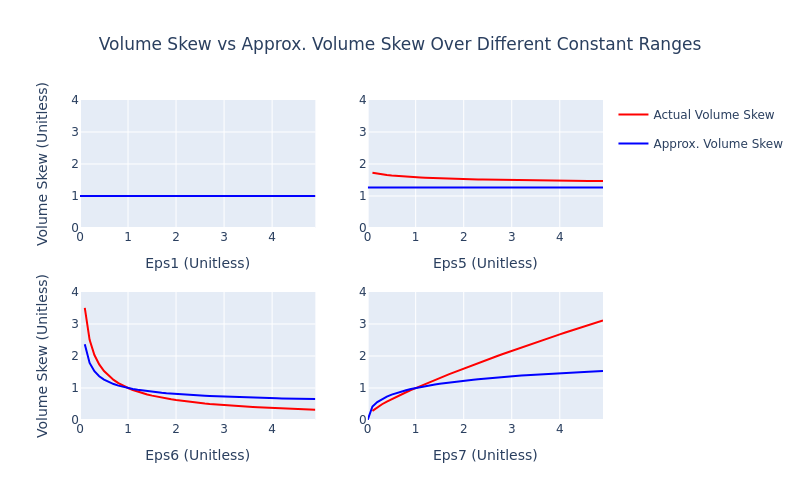
\includegraphics[scale=0.55]{images/ch3/ApproxVsActualVolumeSkew.basic.png}
    \caption{Graphs comparing the approximate and actual volume skew over varrying $\epsilon$ values. Note how the approximation follows the same direction of rate of change of the true volume skew, making it a reasonable approximation for this particular use case.}
    \label{fig:ApproximateVsActualVolumeSkew}
\end{figure}

Before moving on, there has been so much attention on $\epsilon_6$ and $\epsilon_7$ that $\epsilon_5$ has not been discussed, despite having $s$ and $r$ terms associated with it. The constant $\epsilon_5$ represents the volume that should be possible no matter the magnitude of the volume skew. For example, if $\epsilon_6=0$ and $\epsilon_7>0$ for a given exercise, then the following can be stated about the lifter and the way they perform that particular exercise:

\begin{itemize}
    \item The lifter has a volume skew towards reps.
    \item As the lifter leaves there normal volume skew, they should still be able to perform volume in proportion to $\epsilon_5$ even when $r\to 1$ and the contributions from $\epsilon_7$ diminish.
    \item The volume from $\epsilon_5$ is less than any volume that would have been present if $\epsilon_6>0$ because the relation between $\epsilon_5$ and $\epsilon_6$ is additive.
\end{itemize}

Having this representation for baseline work capacity in the opposing volume skew is important. If it was not present the model would assume when a lifter has a certain volume skew, any volume from the opposing skew would simply not be possible. In reality, this is not the case, some baseline level of volume will always be possible, even in the opposite skew. Do not get this confused with volume tolerance, which represents a maximal volume that a lifter can tolerate rather than a baseline of possible volume.

\section{Analysis of Property 1.b: Volume and Intensity}
\label{sec:PotentialSurfaceAnalysisOfProperty1b}

Unbounded volume occurs when volume continually increases, allowing for the potential surface to ask for an infinite amount of work to be done. This presents a serious issue because this is not possible for a lifter to complete, and is especially problematic considering the purpose of this entire chapter is to establish what is possible and what is not possible. Also, if a surface has unbounded volume then property 1.b is proven to not exhibited by this surface because property 1.b needs a volume tolerance to be reached and not surpassed. It needs to be shown that this potential surface doesn't exhibit unbounded volume, or if it does, to establish the boundary where it occurs so it can be avoided when this surface is used in practice.
%
%If volume can be shown to have a global maximum it can be stated that volume is bounded, or does not increase indefinitely. Proving that volume has a peak will require the gradient of $v$.
%
%\begin{equation*}
%	\nabla v=\left[\begin{matrix}
%		\frac{\partial v}{\partial E} \\
%		\frac{\partial v}{\partial F_l} \\
%		\frac{\partial v}{\partial F_w} \\
%		\frac{\partial v}{\partial F_e} \\
%		\frac{\partial v}{\partial s} \\
%		\frac{\partial v}{\partial r} \\
%	\end{matrix}\right]=
%	\left[\begin{matrix}
%		\epsilon_1 \\
%		-\epsilon_2 \\
%		-\epsilon_3 \\
%		-\epsilon_4 \\
%		-2s\left(\epsilon_5(r-1)^2-\epsilon_6\right)+2\epsilon_5(r-1)^2-2\epsilon_6 \\
%		-2r\left(\epsilon_5(s-1)^2-\epsilon_7\right)+2\epsilon_5(s-1)^2-2\epsilon_7 \\
%	\end{matrix}\right]
%\end{equation*}

Rather than trying to prove that volume has a global maximum, it will be shown that 

To prove volume has a peak requires the first partial and second partial derivative of $v$. The partial derivative with respect to $s$ was chosen. It will be discussed later what changes when the partial derivative with respect to $r$ is chosen instead.

\begin{equation}
    \label{eq:IntensitySubedInVolume}
    v(s,r,E)=sr\left( d-a(s-1)^2(r-1)^2-b(s-1)^2-c(r-1)^2-\epsilon E \right)
\end{equation}
\begin{equation}
    \label{eq:VolumeSPartialDerivative}
    \frac{\partial v}{\partial s}=rd-r\epsilon E-cr(r-1)^2-r\left( a(r-1)^2+b \right)\left( 3s^2-4s+1 \right)
\end{equation}
\begin{equation}
    \label{eq:VolumeSSecondPartialDerivative}
    \frac{\partial v'}{\partial s}=-(r)\left( a(r-1)^2+b \right)(6s-4)
\end{equation}

A global maximum occurs when $\partial_{ss} v<0$. In order for this to be the case an even number of the above parenthetical groupings need to be negative. The first parenthetical grouping is always guaranteed to be greater than $1$ from the constraints placed on $r$ in section \ref{sec:UnitsOfMeasurement}. The last parenthetical grouping will be $>0$ if $s>\frac{2}{3}$, which is again guaranteed to be true because of the constraints placed on $s$ in section \ref{sec:UnitsOfMeasurement}. This guarantees two of the three parenthetical groupings to be positive, which forces the middle parenthetical grouping to be positive for $\partial_{ss} v$ to be $<0$. The sign of $a$ changes the set of inequalities that define when the middle parenthetical group is $>0$, and hence when a maximum can occur. Table \ref{tab:BoundedVolumeRanges} shows the inequalities and ranges when volume is bounded for various values of $a$ and $b$.

Care has to be taken when $a=0$ or $b=0$, as the behavior of the inequalities is not fully captured by substituting $0$ for $a$ or $b$. A traditional limit cannot be used because inequalities are one sided, and a limit expects a continuous function. Instead, the four scenarios where $a=0$ and $b=0$ will be treated as one sided limits which will be approached from the side where the behavior is already known. By doing this, the sign can be inferred and the one sided nature of the problem can be handled. \footnote{The notation used in table \ref{tab:BoundedVolumeRanges} is as follows: given a number $x$, $x^-$ is a smaller number approaching $x$, and $x^+$ is a larger number approaching $x$. This allows for one sided analysis to be completed.} The scenarios where the root is imaginary are also troublesome. However, the same one sided analysis can be extended and used again. Looking at table \ref{tab:BoundedVolumeRanges} it should be clear how the one sided limit works as well as how the ranges over which volume is bounded respond.

\begin{table}[h]
    \centering
    \begin{tabular}{c|p{6cm}|c}
        Values for $a$ and $b$ & Inequalities & Range Where Volume is Bounded \\
        \hline

        $a>0$ and $b<0$
        &
        $r> \left(-\frac{b}{a}\right)^\frac{1}{2}+1$
        \newline
        $r< -\left(-\frac{b}{a}\right)^\frac{1}{2}+1$
        &
        $\left( r>\left| \frac{b}{a} \right|^\frac{1}{2}+1 \right) \cup \left( r< -\left| \frac{b}{a} \right|^\frac{1}{2}+1 \right)$
        \\
        \hline
        
        $a>0$ and $b=0$
        &
        $r> \left(-\frac{0^-}{a}\right)^\frac{1}{2}+1$
        \newline
        $r< -\left(-\frac{0^-}{a}\right)^\frac{1}{2}+1$
        &
        $\left( r> 1^+ \right) \cup \left( r<1^- \right)$, a.k.a. $r\ne 1$
        \\
        \hline
        
        $a>0$ and $b>0$
        &
        $r> (0+\beta i)+1$
        \newline
        $r< (-0-\beta i)+1$
        &
        $(r>1)\cup (r<1)$ a.k.a. All $r$
        \\
        \hline
        
        $a=0$ and $b>0$
        &
        $r> \left(-\frac{b}{0^+}\right)^\frac{1}{2}+1=(0+\infty i)+1$
        \newline
        $r< -\left(-\frac{b}{0^+}\right)^\frac{1}{2}+1=(-0-\infty i)+1$
        &
        $(r>1)\cup (r<1)$ a.k.a. All $r$
        \\
        \hline
        
        $a<0$ and $b>0$
        &
        $r< \left(-\frac{b}{a}\right)^\frac{1}{2}+1$
        \newline
        $r> -\left(-\frac{b}{a}\right)^\frac{1}{2}+1$
        &
        $-\left| \frac{b}{a} \right|^\frac{1}{2}+1 < r< \left| \frac{b}{a} \right|^\frac{1}{2}+1$
        \\
        \hline
        
        $a<0$ and $b=0$
        &
        $r< \left(-\frac{0^+}{a}\right)^\frac{1}{2}+1$
        \newline
        $r> -\left(-\frac{0^+}{a}\right)^\frac{1}{2}+1$
        &
        $1^- < r< 1^+$, a.k.a. Never
        \\
        \hline
        
        $a<0$ and $b<0$
        &
        $r< (0+\beta i)+1$
        \newline
        $r> (-0-\beta i)+1$
        &
        $1<r<1$ a.k.a. Never
        \\
        \hline
        
        $a=0$ and $b<0$
        &
        $r< \left(-\frac{b}{0^-}\right)^\frac{1}{2}+1=(0+\infty i)+1$
        \newline
        $r> -\left(-\frac{b}{0^-}\right)^\frac{1}{2}+1=(-0-\infty i)+1$
        &
        $1<r<1$ a.k.a. Never
        \\
    \end{tabular}
    \caption{Various values for $a$ and $b$ as well as there resulting ranges where volume is bounded.}
    \label{tab:BoundedVolumeRanges}
\end{table}

Given the ranges where a maximum could occur, a critical point is still needs to be found, which will require setting $\partial_sv$ equal to $0$. After algebraic manipulation, equation \ref{eq:VolumeRidgeConstR} is generated.
%Using the quadratic formula and substituting $\alpha_s$ in place of the fraction for ease of writing, the following points are generated as critical points.

%the equation below is generated.
\begin{equation}
    \label{eq:VolumeRidgeConstR}
    3s^2-4s+\left( 1-\frac{d-c(r-1)^2-\epsilon E}{a(r-1)^2-b} \right)=0
\end{equation}

 Using the quadratic formula and substituting $\alpha_s$ in place of the fraction for ease of writing, the following points are generated as critical points.
 
\begin{equation*}
    s=\frac{2\pm \sqrt{1+3\alpha_s}}{3}
\end{equation*}

From here the determinant can be used to show where critical points well occur.

\begin{enumerate}
    \item $\alpha_s < -\frac{1}{3}$: No critical points
    \item $\alpha_s = -\frac{1}{3}$: Indeterminate critical point
    \item $\alpha_s > -\frac{1}{3}$: Two critical points
\end{enumerate}

Given the above scenarios for critical points, only option $(3)$ is of interest. As shown below, if $\alpha_s> -\frac{1}{3}$ one critical point is generated on either side of $s=\frac{2}{3}$, the exact $s$ boundary where $\partial_{ss} v$ changes sign. Again, $\partial_{ss} v$ needs to $<0$ for a maximum to be found, requiring the parenthetical relating to $s$ in $\partial_{ss} v$ to be $>0$. This further narrows down the critical points to only include the one that is $>\frac{2}{3}$. It is worth mentioning that this is also the only valid critical point from the context of the problem, with $s$ being constrained to be $>1$ in section \ref{sec:UnitsOfMeasurement}.

\begin{equation*}
    s=\frac{2\pm \sqrt{1+3\left( -\frac{1}{3} \right)^+}}{3}=\frac{2\pm 0^+}{3}=\left( \frac{2}{3} \right)^-, \left( \frac{2}{3} \right)^+
\end{equation*}

Given that $\alpha_s>-\frac{1}{3}$, there will be a critical point. This can now be combined with the ranges where volume is bounded as well as the context of the problem to create the following statements:

\begin{enumerate}
    \item Volume is fully bounded for all $r$ when $a,b>0$.
    \item When $a>0$ and $b=0$ volume is fully bounded for all $r\ne 1$.
    \item When $a<0$ and $b=0$ volume is never bounded.
    \item When $a=0$ and $b>0$, volume is fully bounded.
    \item When $a=0$ and $b<0$, volume is never bounded.
    \item When $a>0$ and $b<0$, volume is bounded for $r>\left| \frac{b}{a} \right|^\frac{1}{2}+1$.
    \item When $a<0$ and $b>0$, volume is bounded for $1\le r < \left| \frac{b}{a} \right|^\frac{1}{2}+1$
\end{enumerate}

This analysis only looked at sets, which was an assumption made from the very beginning when the partial derivative of $v$ was taken with respect to $s$. If instead, the partial derivative was taken with respect to $r$, an analogous process would be followed. Due to the symmetry from $\partial_sv$ and $\partial_rv$, the only differences will be $c$ replacing $b$, $\alpha_r$ replacing $\alpha_s$ and, obviously, $s$ and $r$ switching roles. This creates the following additional statements given that $\alpha_r>-\frac{1}{3}$:

\begin{enumerate}
    \setcounter{enumi}{7}
    \item Volume is fully bounded for all $s$ when $a,c>0$.
    \item When $a>0$ and $c=0$ volume is fully bounded for all $s\ne 1$.
    \item When $a<0$ and $c=0$ volume is never bounded.
    \item When $a=0$ and $c>0$, volume is fully bounded.
    \item When $a=0$ and $c<0$, volume is never bounded.
    \item When $a>0$ and $c<0$, volume is bounded for $s>\left| \frac{c}{a} \right|^\frac{1}{2}+1$.
    \item When $a<0$ and $c>0$, volume is bounded for $1\le s < \left| \frac{c}{a} \right|^\frac{1}{2}+1$
\end{enumerate}

For peace of mind, figure \ref{fig:VolumeConstSRPeak} shows the peak volume identified by the above algebraic analysis. There is a peak for all $s$ and $r$ values, which means that volume is fully bounded. This also matches the statements above as $a=1.6\times 10^{-4}$, $b=2.7\times 10^{-3}$, and $c=2.9\times 10^{-3}$, which are all greater than $0$.

\begin{figure}[h]
    \centering
    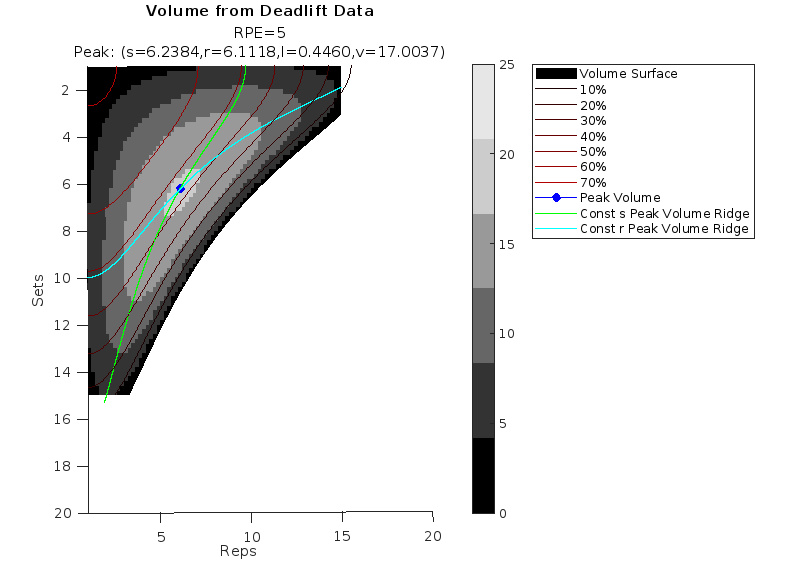
\includegraphics[width=170mm]{DeadliftVolume/FailedRidgeIdentification-2.png}
    \caption{The peak identified in volume given constant $s$ and $r$ values. This may look similar to figure \ref{fig:DeadliftIntensityCriticalPointsOnVolume} but they are two different graphs that were generated from two different approaches.}
    \label{fig:VolumeConstSRPeak}
\end{figure}

The above statements make sense in isolation, but when considered together things can contradict each other. If $a<0$, $b=0$, and $c>0$, then  statement $(3)$ states volume is never bounded, but statement $(14)$ states volume is bounded for a specific region. Again, this is the result of looking at a three dimensional problem from two dimensions, and is the same reason why the two peak volume lines in figure \ref{fig:VolumeConstSRPeak} do not coincide. While this does create some problems, the above statements are still is able to give some intuition for the problem at hand. Revisiting the example stated previously, it is saying that volume from reps is never bounded, and volume from sets is only bounded over a region. This intuition can be used to adjust training appropriately to avoid unbounded volume.

It is tempting to say the bounds in the above statements can be used in practice to limit the lifter from doing to much volume, but just because volume is bounded does not mean it is reasonable. Just because it can be proven that volume has a peak does not prove that the peak volume is attainable. This is a limitation of the model that stems from using linear regression to fit a surface to the data. Linear regression will implicitly extrapolate what amount of volume can be done given the data it has. Extrapolation is a known weakness of linear regression, making its predicted volume sometimes inaccurate.

To simplify the model, $b$ and $c$ can be limited to being $\ge 0$ so that volume will only ever be unbounded when $b=0$ or $c=0$. Not only does this remove the complexities of defining ranges over which the potential surface has bounded volume, but it makes intuitive sense to limit the model to only describing what is possible.


%
%\section{Analysis: Proving Volume Increases With Weight Until a Peak Is Reached}
%\label{sec:PotentialSurfaceVolumePeak}
%
%It needs to be shown that, given a constant effort, volume increases with weight until a peak is reached at which point volume decreases. Analytically, this translates to finding the critical points and concavity of the volume equation. After solving equation \ref{eq:PotentialSurfaceEquation} for $s$ and substituting it in equation \ref{eq:IntensityBasedVolumeEquation}, equation \ref{eq:SetsSubedInVolume} is created and the process of finding critical points can be started. For simplicity, the volume equation will be scaled by $l_{1RM}$, removing its presence on the right hand side of the equation. The first and second partial derivatives of $v$ with respect to $I$ will also be needed.
%
%\begin{equation}
%    \label{eq:SetsSubedInVolume}
%    v(r,I,E)=rI\left( \left( \frac{d-I-c(r-1)^2-\epsilon E}{a(r-1)^2+b} \right)^\frac{1}{2} +1 \right)
%\end{equation}
%\begin{equation}
%    \label{eq:VolumeIPartialDerivative}
%    \frac{\partial v}{\partial I} = 
%    r+
%    r\left( a(r-1)^2+b \right)^{-\frac{1}{2}} 
%    \left( d-I-c(r-1)^2-\epsilon E \right)^\frac{1}{2}
%    \left(
%        1-\frac{I}{2}\left( d-I-c(r-1)^2-\epsilon E \right)^{-\frac{3}{2}}
%    \right)
%\end{equation}
%\begin{equation}
%    \label{eq:VolumeISecondPartialDerivative}
%    \frac{\partial v'}{\partial I}=
%    -r\left( a(r-1)^2+b \right)^{-\frac{1}{2}}
%    \left( d-I-c(r-1)^2-\epsilon E \right)^{-\frac{1}{2}}
%    \left(
%        1+\frac{I}{4}\left( d-I-c(r-1)^2-\epsilon E \right)^{-1}
%    \right)
%\end{equation}
%
%Both $\partial_Iv$ and $\partial_{II}v$ will need to be set to $0$ and solved for. When looking at $\partial_{II}v$, in order for a maximum to occur $\partial_{II}v<0$. Looking at the parenthetical groups of $\partial_{II}v$, the first two are guaranteed to be $\ge 0$.
%
%\begin{enumerate}
%    \item $r\ge0$ from section \ref{sec:UnitsOfMeasurement}
%    \item $\left( a(r-1)^2+b \right)^{-\frac{1}{2}}>0$ from section \ref{sec:UnitsOfMeasurement} and the constraints placed on $a$ and $b$ in equation \ref{eq:PotentialSurfaceEquation}
%\end{enumerate}
%
%The third parenthetical group creates a further constraint for the current problem in question, and is shown in the inequality below. This constraint guarantees that the third parenthetical group is $>0$.
%
%\begin{equation*}
%    d-I-c(r-1)^2-\epsilon E>0
%\end{equation*}
%
%Given that the first three parenthetical groups are all $>0$, the last one must also be $>0$ in order for $\partial_{II}v$ to be $<0$. The inequality from the fourth parenthetical grouping is shown below. The constraint above nicely eliminates the imaginary part of the inequality.
%
%\begin{equation*}
%    I<\frac{4}{3}\left( d-c(r-1)^2-\epsilon E \right)
%\end{equation*}
%
%Before moving on, it is worth exploring what the above inequality has to say. As $r$ increases the range over which a maximum can occur in $I$ decreases. This may seem counter intuitive, but when considered from the perspective of volume it makes more sense. At the extreme, as the number of reps continue to increase volume continues to increase, which necessitates weight decreasing, making $I$ decrease. This is important because it shows the model respects the limitations that volume presents on weight.
%
%Given the range where a maximum can occur, a critical point still needs to be found. This is not so easily done, and requires a computational approach. Using deadlift data, figure \ref{fig:DeadliftIntensityCriticalPoints} shows where the critical points are in relation to the region where a maximum can occur. It is clear that the critical points are all within the appropriate region to guarantee a maximum occurs.
%
%\begin{figure}
%    \centering
%    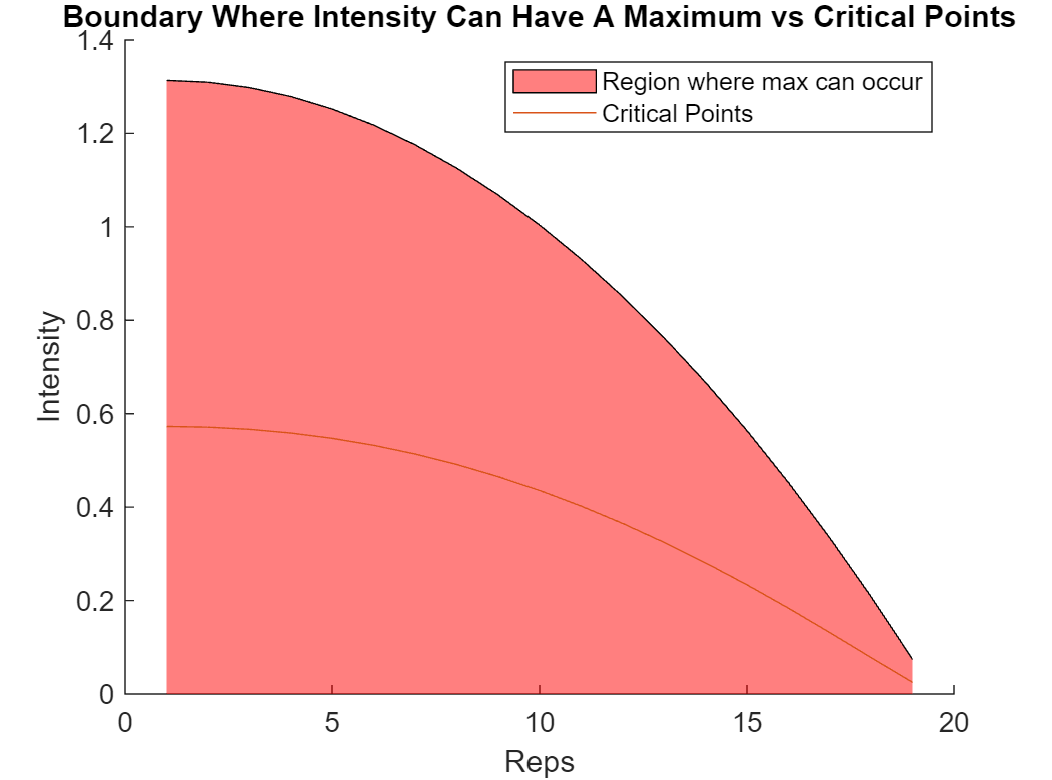
\includegraphics[width=140mm]{DeadliftConstants/IntensityCriticalPoints.png}
%    \caption{Critical points for intensity from deadlift data and a time frame of 120 days with an effort of $E=5$. Note how they are all within the boundary where a maximum can occur.}
%    \label{fig:DeadliftIntensityCriticalPoints}
%\end{figure}
%
%Before carrying on, it is worth mentioning that the same process used to find intensity critical points can be carried out but instead of solving equation \ref{eq:PotentialSurfaceEquation} for $s$, it can be solved for $r$. Doing this produces analogous analytical results, with $b$ and $c$ switching places along with $s$ and $r$. In order for the true peak in $I$ to be found, both approaches need to correspond to the same set of critical points. To help visualize any differences, the two sets of critical points can be plotted on top of the volume surface, as shown in figure \ref{fig:DeadliftIntensityCriticalPointsOnVolume}. From this figure, it should be clear that the two different ways to identify the peak in $I$ do not produce the same result.
%
%\begin{figure}
%    \centering
%    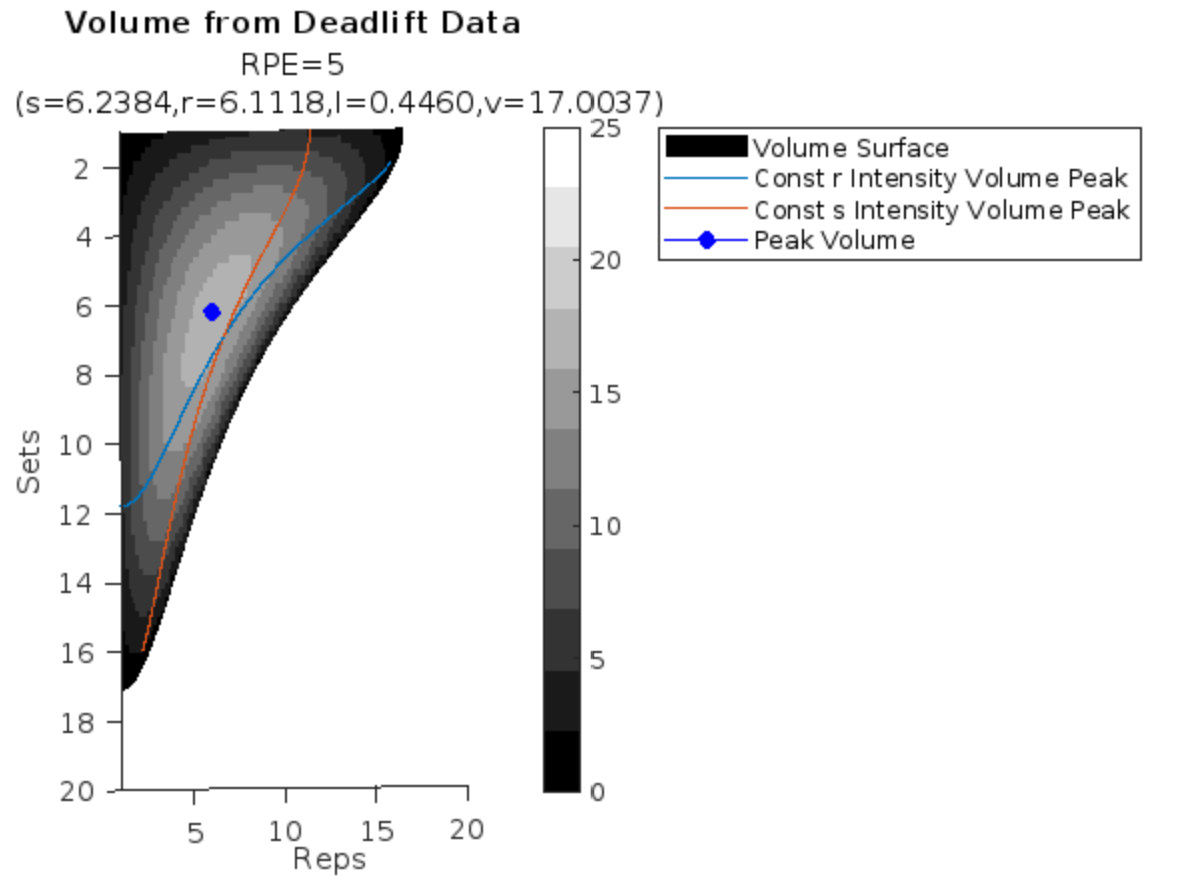
\includegraphics[width=140mm]{DeadliftConstants/IntensityCriticalPointsOnVolume.png}
%    \caption{Intensity critical points graphed on the volume surface. These lines represent where intensity is maximized, in relation to constant $s$ and $r$ values.}
%    \label{fig:DeadliftIntensityCriticalPointsOnVolume}
%\end{figure}
%
%The reason for the discrepancies in results can be explained by simplifying the problem to two dimensional approaches. The original three dimensional problem was reduced down to two different two dimensional problems, creating two separate ways to view the problem, and hence two different solutions. With an analytical approach failing to create consistent results, the graphs in table \ref{tab:DeadliftVolumeAcrossEffortOnlyIntensity} serve as the best proof that volume increases with effort until a peak is reached. These graphs do show some of the problems of viewing the problem from two dimensions. They show that volume does not always increase or decrease across intensity for all values of $r$. What does appear to increase across $I$ until a peak is reached is the peak volume.
%
%\begin{table}
%    \centering
%    \begin{tabular}{c|c}
%        RPE & Volume Across Intensities \\
%        \hline
%        
%        5 &
%        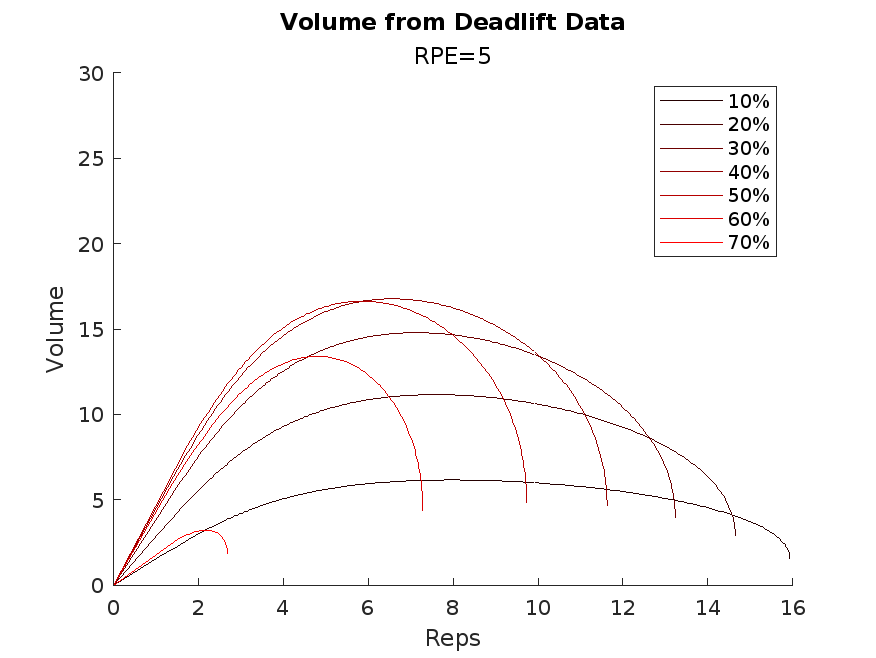
\includegraphics[width=140mm]{DeadliftVolume/5-2.png} \\
%        
%        %8 &
%        %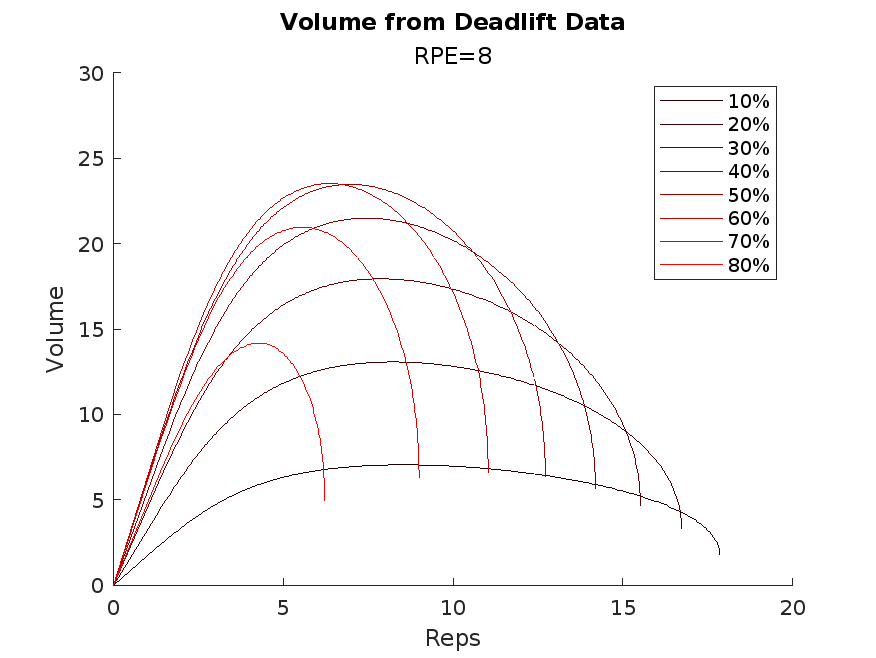
\includegraphics[width=76mm]{DeadliftVolume/8-2.png} \\
%        
%        10 &
%        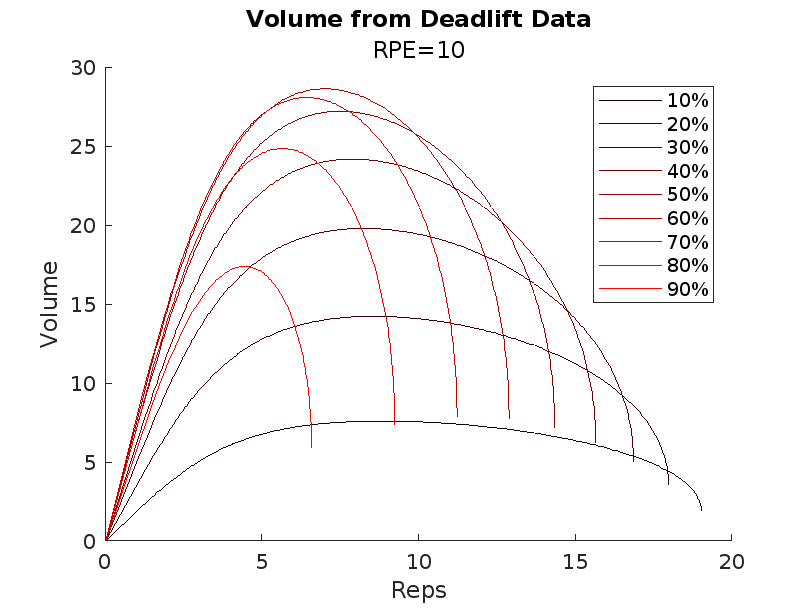
\includegraphics[width=140mm]{DeadliftVolume/10-2.png} \\
%    \end{tabular}
%    \caption{The same volume equation from table \ref{tab:DeadliftVolumeAcrossEffort} but only graphed across different intensities. Again, the vertical axis scaled by $l_{1RM}$. The intensity lines on the graphs in table \ref{tab:DeadliftVolumeAcrossEffort} correspond to the same intensity lines on these graphs.}
%    \label{tab:DeadliftVolumeAcrossEffortOnlyIntensity}
%\end{table}
%
%
%
%\section{Application: Solving for the Unknown}
%\label{sec:PotentialSurfaceSolvingForTheUnknown}
%
%With the model presented so far, one of the variables can be solved for given some combination of sets, reps, effort, or weight. This is useful because it can give a lifter information they otherwise would have guessed. Equations \ref{eq:PotentialSurfaceSetsEquation} through \ref{eq:PotentialSurfaceEffortEquation} are the potential surface solved for various variables.
%
%\begin{subequations}
%    \begin{align}
%        s(r,I,E)&=
%        \left( 
%            \frac{
%                d-I-c(r-1)^2-\epsilon E
%            }{
%                a(r-1)^2+b
%            }
%        \right)^\frac{1}{2}+1
%        \label{eq:PotentialSurfaceSetsEquation}\\
%        r(s,I,E)&=
%        \left(
%            \frac{
%                d-I-b(s-1)^2-\epsilon E
%            }{
%                a(s-1)^2+c
%            }
%        \right)^\frac{1}{2}+1
%        \label{eq:PotentialSurfaceRepsEquation}\\
%        I(s,r,E)&=
%        d-a(s-1)^2(r-1)^2-b(s-1)^2-c(r-1)^2-\epsilon E
%        \label{eq:PotentialSurfaceIntensityEquation}\\
%        E(s,r,I)&=
%        \frac{
%            d-I-a(s-1)^2(r-1)^2-b(s-1)^2-c(r-1)^2
%        }{
%            \epsilon
%        }
%        \label{eq:PotentialSurfaceEffortEquation}
%    \end{align}
%\end{subequations}
%
%As an example of using the above equations, a lifter is often concerned with estimating an updated 1RM for an exercise after completing some training. Increases in weight for a lifts 1RM is a sign of progress and successful training. The model presented already estimates a users current 1RM, just in a round-about way. A 1RM will be a maximal effort lift with one set of one rep. Given these parameters, the weight lifted can be found using equation \ref{eq:PotentialSurfaceIntensityEquation}, which can just be multiplied by the weight of the lifters known 1RM to get the weight of the lifters predicted 1RM, as shown in equation \ref{eq:1RMPrediction}.
%
%\begin{equation}
%    \label{eq:1RMPrediction}
%    n_{1RM}=I(s=1,r=1,E=10)l_{1RM}=l_{1RM}( d-10\epsilon )
%\end{equation}
%
%It is worth taking a step back to understand what equation \ref{eq:1RMPrediction} is saying. The new 1RM is generated from a baseline value, $d$, which increases with effort, $10\epsilon$. \footnote{Remember, $\epsilon$ needs to be $<0$ for the model to behave appropriately. This was discussed in section \ref{sec:PotentialSurfaceVolumeIncreasesWithEffort}.} This intuitively makes sense, as the more effort a lifter exerts the greater there 1RM is should be.
%
%To test the accuracy of equation \ref{eq:1RMPrediction}, the model can be made to fit to data before a 1RM attempt and then compare the predicted 1RM to the actual 1RM. The lifter had two competitions where 1RM's were tested: the first was deadlift only and the second was a full meet. The predicted and actual 1RM's for all the exercises performed at each competition are summarized in table \ref{tab:1RMPredictedVsActual}.
%
%\begin{table}[h]
%    \centering
%    \begin{tabular}{p{2cm}|p{2cm}|p{2cm}|p{2cm}|p{2cm}|p{2cm}|p{2cm}}
%        Exercise & Date & Time Frame (Days) & Current Time (Days) & Predicted 1RM (lbs) & Actual 1RM (lbs) & Difference (lbs) \\
%        \hline
%        
%        Deadlift & 5/5/2022 & $40$ & $81$ & $506$ & $520$ & $14$ \\
%        Squat & 7/24/2022 & $120$ & $1$ & $415$ & $435$ & $20$ \\
%        Bench & 7/24/2022 & $120$ & $1$ & $267$ & $270$ & $3$ \\
%        Deadlift & 7/24/2022 & $120$ & $1$ & $511$ & $535$ & $24$ \\
%    \end{tabular}
%    \caption{Predicted vs actual 1RM's. All weight values are rounded to the nearest pound.}
%    \label{tab:1RMPredictedVsActual}
%\end{table}
%
%The model consistently under-predicts the lifters 1RM, and the largest difference in the predicted vs actual 1RM is $24$ lbs. The smallest difference is $3$ lbs. The time frames were chosen to limit the data to only data points after $3/27/2022$, which is the date of the first successful workout after the lifter sustained an injury and took two weeks off from the gym entirely. Section \ref{sec:PotetentialSurfaceImprovingAccuracy} will work towards improving the accuracy of the predicted 1RM.
%
%%As with section \ref{sec:PotentialSurfaceAbstractlyDescribingTraining}, a lifters 1RM can be tracked across time, providing another way to describe training over time. Figure \ref{fig:Deadlift1RMOverTime} shows the models predicted 1RM over time. Again, while presented here as an application of the model, more will be gained from figure \ref{fig:Deadlift1RMOverTime} in section \ref{sec:Macrocycle}.
%%
%%\begin{figure}[h]
%%    \centering
%%    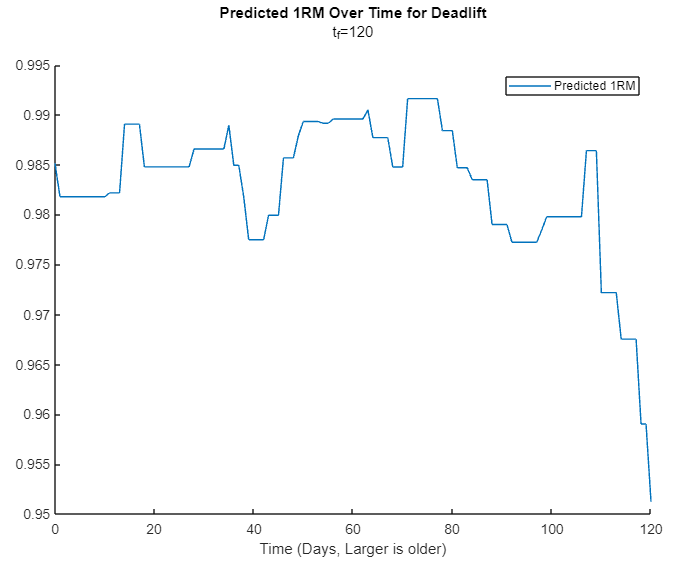
\includegraphics[width=140mm]{DeadliftConstants/pred1RM.png}
%%    \caption{The models predicted 1RM over time for deadlift.}
%%    \label{fig:Deadlift1RMOverTime}
%%\end{figure}
%
%\section{Improving Accuracy: Improvising for What's Not Included}
%\label{sec:PotetentialSurfaceImprovingAccuracy}
%
%Fatigue was presented in section \ref{sec:CommonTermsSection}, but until this point was not considered. This is mainly because it is not part of the data set that was used to generate the potential surface. Fatigue directly limits what can be lifted. This makes intuitive sense: a lifter that is fatigued will be tired and hence will not able to lift as much weight. This is one of the reasons why it gets harder to lift a given weight the more times it is attempted. Given this, if fatigue were to be added to the model it may look like something like equation \ref{eq:PotentialSurfaceEquationWithFatigue}, where $F$ is used to represent fatigue.
%
%\begin{equation}
%    \label{eq:PotentialSurfaceEquationWithFatigue}
%    a(s-1)^2(r-1)^2+b(s-1)^2+c(r-1)^2+\epsilon E+\epsilon_2 F=d-I
%\end{equation}
%
%While fatigue cannot be represented directly by the model due to it not being part of the data, its affects should still be sought to be minimized. Within the broad category of fatigue, there two sub-types: \textit{inter-workout} and \textit{inter-exercise} fatigue. As the names suggest, inter-workout fatigue is fatigue that accumulates over the course of an entire workout, and inter-exercise fatigue is fatigue that accumulates over the course of a single exercise. When a lifter switches exercises fatigue drops depending on the amount of similarity between the exercises. If two exercises are similar more fatigue will carry over between them, increasing both the perceived inter-workout fatigue as well as the inter-exercise fatigue on the second exercise. On some occasions this is purposeful, and is used as a way to increase stimulus while keeping intensity low.
%
%It should be obvious that effects from inter-workout fatigue cannot be minimized, as this surface is only defined for a single exercise, but the effects from inter-exercise fatigue can be partially controlled for. If the same exercise is performed on the same day with different weights, then each set with a different weight can be given an 'index' to show the order that the sets occurred in.\footnote{This obviously only includes working sets. Warm up sets will not be indexed.} This order will then take the place of a fatigue measurement, and linear regression can be completed using the augmented data set. While not perfect, this works because the index increases as fatigue would increase, creating a way to test if having actual fatigue data would increase the accuracy of the model. This 'index' will be called the \textit{fatigue index} and will will start at $0$ to reflect that the first set done will have no fatigue. If the value for $\epsilon_2$ from linear regression is not near $0$ then it can be said fatigue significantly contributes to the model. Table \ref{tab:LinearRegressionConstantsWithFatigue} shows the results after completing linear regression on deadlift data with the new augmented data set. It is clear, when compared to the other constants, the $\epsilon_2$ constant is large enough to be significant.
%
%\begin{table}[h]
%    \centering
%    \begin{tabular}{c|c|c|c|c|c|c}
%         & $a$ & $b$ & $c$ & $d$ & $\epsilon$ & $\epsilon_2$ \\
%         \hline
%        With Fatigue Index & $0.0001$ & $0.0029$ & $0.0028$ & $0.4179$ & $-0.0519$ & $0.0173$ \\
%        Without Fatigue Index & $0.0002$ & $0.0027$ & $0.0029$ & $0.4302$ & $-0.0555$ & - \\
%    \end{tabular}
%    \caption{Linear regression constants from deadlift data with and without the augmented fatigue data.}
%    \label{tab:LinearRegressionConstantsWithFatigue}
%\end{table}
%
%Despite augmenting the data set and adding a new variable, much of the work outlined in sections \ref{sec:PotentialSurfaceVolumeIncreasesWithEffort}-\ref{sec:PotentialSurfaceSolvingForTheUnknown} remains unaffected, as the added fatigue term either drops out after performing differentiation or just tags along similar to the effort term. The changes to equations \ref{eq:PotentialSurfaceSetsEquation}-\ref{eq:PotentialSurfaceEffortEquation} are shown in equations \ref{eq:PotentialSurfaceSetsEquationWithFatigue}-\ref{eq:PotentialSurfaceEffortEquationWithFatigue} for convenience.
%
%\begin{subequations}
%    \begin{align}
%        s(r,I,E,F)&=
%        \left( 
%            \frac{
%                d-I-c(r-1)^2-\epsilon E-\epsilon_2 F
%            }{
%                a(r-1)^2+b
%            }
%        \right)^\frac{1}{2}+1
%        \label{eq:PotentialSurfaceSetsEquationWithFatigue}\\
%        r(s,I,E,F)&=
%        \left(
%            \frac{
%                d-I-b(s-1)^2-\epsilon E-\epsilon_2 F
%            }{
%                a(s-1)^2+c
%            }
%        \right)^\frac{1}{2}+1
%        \label{eq:PotentialSurfaceRepsEquationWithFatigue}\\
%        I(s,r,E,F)&=
%        d-a(s-1)^2(r-1)^2-b(s-1)^2-c(r-1)^2-\epsilon E-\epsilon_2 F
%        \label{eq:PotentialSurfaceIntensityEquationWithFatigue}\\
%        E(s,r,I,F)&=
%        \frac{
%            d-I-a(s-1)^2(r-1)^2-b(s-1)^2-c(r-1)^2-\epsilon_2 F
%        }{
%            \epsilon
%        }
%        \label{eq:PotentialSurfaceEffortEquationWithFatigue}\\
%        F(s,r,I,E)&=
%        \frac{
%            d-I-a(s-1)^2(r-1)^2-b(s-1)^2-c(r-1)^2 -\epsilon E
%        }{
%            \epsilon_2
%        }
%        \label{eq:PotentialSurfaceFatigueEquation}
%    \end{align}
%\end{subequations}
%
%%As equation \ref{eq:PotentialSurfaceFatigueEquation} demonstrates, the fatigue index value can also be solved for, which presents an interesting opportunity to measure how fatigued a lifter is based on there previous lifts. Through equation \ref{eq:PotentialSurfaceEffortEquationWithFatigue}, the model will be able to predict a fatigue index. This fatigue index can then be compared to the actual fatigue index, and the delta can be used to show how fatigued you are compared to what the model expects. Equation \ref{eq:}
%
%The changes to equation \ref{eq:1RMPrediction}, as shown in equation \ref{eq:1RMPredictionWithFatigue}, are also important. With the new predicted 1RM equation, there is still a baseline value, $d$, which increases with effort, $10\epsilon$, but the baseline value now decreases with fatigue, $\epsilon_2 F$. Again, this intuitively makes sense. If a lifter is in a fatigued state, they will not be able to lift as much weight, even with high amounts of effort. Put another way: performance is effort minus fatigue.
% 
%\begin{equation}
%    \label{eq:1RMPredictionWithFatigue}
%    n_{1RM}=I(s=1,r=1,E=10,F)l_{1RM}=l_{1RM}( d-10\epsilon-\epsilon_2 F)
%\end{equation}
%
%The updated 1RM prediction equation can be compared to the old one to see which one is more accurate. Table \ref{tab:Predicted1RMWithAndWithoutFatigue} compares the estimated 1RM's between the augmented data set and the non-augmented data set. The same lifts and time frames are used as table \ref{tab:1RMPredictedVsActual}. When computing the predicted 1RM with fatigue, a fatigue index of $F=0$ was used, as a 1RM attempt is usually the first set performed to avoid any affects from fatigue.
%
%\begin{table}[h]
%    \centering
%    \begin{tabular}{p{2cm}|p{2cm}|p{3cm}|p{3cm}|p{3cm}}
%        Exercise &  Date & Pred. 1RM With $F$  (lbs) & Pred. 1RM Without $F$ (lbs) & Actual 1RM (lbs) \\
%        \hline
%        Deadlift & 5/5/2022 & $506$ & $506$ & $520$ \\
%        Squat & 7/24/2022 & $417$ & $415$ & $435$ \\
%        Bench & 7/24/2022 & $269$ & $267$ & $270$ \\
%        Deadlift & 7/24/2022 & $514$ & $511$ & $535$ \\
%    \end{tabular}
%    \caption{Predicted 1RM with and without the augmented fatigue data.}
%    \label{tab:Predicted1RMWithAndWithoutFatigue}
%\end{table}
%
%As shown in table \ref{tab:Predicted1RMWithAndWithoutFatigue}, when the model is augmented with the fatigue index it has either the same or greater accuracy when predicting a 1RM, especially on bench, with the model being within $1$ pound of the users actual 1RM.
%
%The affects of $\epsilon_2$ on $I$ also need to be considered to ensure the model is appropriately responding to fatigue. As such, the changes in $I$ relating to changes in $F$ are desired, requiring the derivative of equation \ref{eq:PotentialSurfaceEffortEquationWithFatigue} with respect to $F$. 
%
%\begin{equation}
%    \label{eq:VolumeFPartialDerivative}
%    \frac{\partial I}{\partial F}=\frac{\partial}{\partial F} d-a(s-1)^2(r-1)^2-b(s-1)^2-c(r-1)^2-\epsilon E-\epsilon_2 F=-\epsilon_2
%\end{equation}
%
%As stated at the start of this section, fatigue limits what can be lifted. As such, $I$ needs to decrease as $\epsilon_2$ increases, requiring $\partial_F I<0$. It should be obvious that this can only happen if $\epsilon_2>0$, meaning that intensity decreases with fatigue \textbf{iff} $\epsilon_2>0$. Given the values for $\epsilon_2$ in table \ref{tab:Epsilon2AcrossExercises}, which are all positive, it is clear the model is appropriately identifying patterns in fatigue.
%
%\begin{table}[h]
%    \centering
%    \begin{tabular}{c|c}
%        Exercise & $\epsilon_2$ \\
%        \hline
%        Squat & $0.0116$ \\
%        Bench & $0.0301$ \\
%        Deadlift & $0.0173$ \\
%    \end{tabular}
%    \caption{The $\epsilon_2$ values for three different exercises. They are all positive, meaning the model is correctly making intensity decrease with increased fatigue.}
%    \label{tab:Epsilon2AcrossExercises}
%\end{table}
%
%Augmenting the data with the fatigue index clearly improved the accuracy of the model, it is still not perfect. While the fatigue index does have the same general behavior as fatigue, it is not the exact same behavior. One difference is that fatigue will accumulate across all sets, not just across sets with a different weight. If each set was given an increasing fatigue index, regardless of weight, the model would no longer be able to accurately understand sets because every exercise would be split up into a list of single sets with a certain number of reps and an incrementing fatigue index. Splitting the data points apart like this would also create dependencies between the data points, which cannot happen with linear regression. To make sure the model accurately understands the relation between sets and reps, the fatigue index was made to only increase across sets of different weight. This has the unfortunate side effect of giving the fatigue index behavior that fatigue does not have, but is necessary to keep the rest of the model consistent.
%
%All this consideration with the fatigue index raises the question: why not just create a new data set that records fatigue? Arguably, using actual fatigue data would give better results. The problem is that fatigue is hard to measure. A simple system like RPE cannot be used because often times a lifter may by psychologically fatigued, but physically they are fine, or visa versa. As John Broz, an Olympic trainer, says, "How you feel is a lie." While John has an extreme take on the discrepancy between how a lifter feels and how they perform, there is still some level of truth to the statement. There are many cases where a lifters psychological state does not match there physical state, resulting in discrepancies between what they think they can do and what they actually do during a workout. As such, simply asking a lifter to record how fatigued they feel on a given day is not going to produce reliable data. Other methods of measuring fatigue exist\cite{MEASURING_FATIGUE}, but these methods are generally not conducive to a training environment, which is where they would need to be used to capture changes in fatigue across sets. Finding a way to reliably record fatigue data while training will remain an unanswered question.
%
%Due to the increased accuracy of the model with the fatigue index added to the data set, the rest of the paper will continue to use this updated model, which will be called the \textit{fatigue aware potential surface}.
%
%%This is promising, and all seems well until volume skew is considered. Looking at $b$ and $c$ in table \ref{tab:LinearRegressionConstantsWithFatigue}, it should be obvious that the volume skew shifted. The volume skew without $F$ is $0.9495$, but with $F$ it is $1.0361$. Remembering the definition of volume skew, this means volume went from favoring sets to favoring reps. Looking at the graph from the raw data in figure \ref{fig:SetsVsReps} it should be clear the the model should favor sets, not reps.
%
%%\section{Time Frame Considerations}
%%\label{sec:PotentialSurfaceTimeFrameConsiderations}
%
